%%%%%%%% NEURIPS 2024 EXAMPLE LATEX SUBMISSION FILE %%%%%%%%%%%%%%%%%


\documentclass{article}


\usepackage[utf8]{inputenc} % allow utf-8 input
\usepackage[T1]{fontenc}    % use 8-bit T1 fonts
\usepackage{hyperref}       % hyperlinks
\usepackage{url}            % simple URL typesetting
\usepackage{booktabs}       % professional-quality tables
\usepackage{amsfonts}       % blackboard math symbols
\usepackage{nicefrac}       % compact symbols for 1/2, etc.
\usepackage{microtype}      % microtypography
\usepackage{xcolor}         % colors

% Recommended, but optional, packages for figures and better typesetting:
\usepackage{graphicx}
\usepackage{subfig}
\usepackage{adjustbox}
\usepackage{booktabs} % for professional tables
% hyperref makes hyperlinks in the resulting PDF.
% If your build breaks (sometimes temporarily if a hyperlink spans a page)
% please comment out the following usepackage line and replace
% \usepackage{icml2024} with \usepackage[nohyperref]{icml2024} above.
% Attempt to make hyperref and algorithmic work together better:
\newcommand{\theHalgorithm}{\arabic{algorithm}}
% Use the following line for the initial blind version submitted for review:

% If accepted, instead use the following line for the camera-ready submission:
\usepackage[accepted]{icml2024}

\usepackage{wrapfig}

\usepackage{dblfloatfix}% http://ctan.org/pkg/dblfloatfix
\usepackage{lipsum}% http://ctan.org/pkg/lipsum

\def\R{\mathbb{R}}
\def\N{\mathbb{N}}
\def\C{\mathbb{C}}
\def\d{\partial}
\newcommand{\bd}[1]{{\bf #1}}
\newcommand{\dd}[2]{\frac{\partial #1}{\partial #2}}

\newcommand{\eq}[1]{\begin{equation}
    \begin{split}
        #1
    \end{split}
\end{equation}}
\newcommand{\eqbox}[1]{\begin{equation}
    \boxed{
    \begin{split}
        #1
    \end{split}
    }
\end{equation}}

% For theorems and such
\usepackage{amsmath}
\usepackage{physics}
\usepackage{amssymb}
\usepackage{mathtools}
\usepackage{amsthm}
\DeclareMathOperator*{\argmin}{arg\,min}
\def\d{\partial}

% if you use cleveref..
\usepackage[capitalize,noabbrev]{cleveref}

%%%%%%%%%%%%%%%%%%%%%%%%%%%%%%%%
% THEOREMS
%%%%%%%%%%%%%%%%%%%%%%%%%%%%%%%%
\theoremstyle{plain}
\newtheorem{theorem}{Theorem}[section]
\newtheorem{proposition}[theorem]{Proposition}
\newtheorem{lemma}[theorem]{Lemma}
\newtheorem{corollary}[theorem]{Corollary}
\theoremstyle{definition}
\newtheorem{definition}[theorem]{Definition}
\newtheorem{assumption}[theorem]{Assumption}
\theoremstyle{remark}
\newtheorem{remark}[theorem]{Remark}

% Todonotes is useful during development; simply uncomment the next line
%    and comment out the line below the next line to turn off comments
%\usepackage[disable,textsize=tiny]{todonotes}
\usepackage[textsize=tiny]{todonotes}

\newcommand{\simcom}[1]{\textcolor{blue}{[SM: #1]}}

% The \icmltitle you define below is probably too long as a header.
% Therefore, a short form for the running title is supplied here:


\begin{document}

\twocolumn[
\icmltitle{Extending Surrogate Hamiltonian Monte Carlo}

% It is OKAY to include author information, even for blind
% submissions: the style file will automatically remove it for you
% unless you've provided the [accepted] option to the icml2024
% package.

% List of affiliations: The first argument should be a (short)
% identifier you will use later to specify author affiliations
% Academic affiliations should list Department, University, City, Region, Country
% Industry affiliations should list Company, City, Region, Country

% You can specify symbols, otherwise they are numbered in order.
% Ideally, you should not use this facility. Affiliations will be numbered
% in order of appearance and this is the preferred way.
\icmlsetsymbol{equal}{*}

\begin{icmlauthorlist}
\icmlauthor{Abhijit Brahme}{equal,statistics}


%\icmlauthor{}{sch}
\end{icmlauthorlist}

\icmlaffiliation{statistics}{Department of Statistics, University of California, Santa Barbara, USA}


\icmlcorrespondingauthor{Abhijit Brahme}{abhijitbrahme@ucsb.edu}


% You may provide any keywords that you
% find helpful for describing your paper; these are used to populate
% the "keywords" metadata in the PDF but will not be shown in the document
\icmlkeywords{Machine Learning, ICML, Hamiltonian Monte Carlo, Neural ODE, Symplectic}

\vskip 0.3in
]

% this must go after the closing bracket ] following \twocolumn[ ...

% This command actually creates the footnote in the first column
% listing the affiliations and the copyright notice.
% The command takes one argument, which is text to display at the start of the footnote.
% The \icmlEqualContribution command is standard text for equal contribution.
% Remove it (just {}) if you do not need this facility.

%\printAffiliationsAndNotice{}  % leave blank if no need to mention equal contribution


% We combine tools from Lie theory and differential geometry to develop a novel algorithm for reconstructing a spatially varying metric tensor from trajectory valued data. We show through synthetic examples that this approach is robust to noise, flexible enough to encode various symmetries, and performs well in situations with sparse data. 
\begin{abstract}
The advent of automatic differentiation \cite{baydin2018automatic} has allowed gradient based MCMC methods to prosper. For example, Hamiltonian Monte Carlo \cite{Brooks_2011} (HMC) has been the workhorse of Bayesian inferential methods, allowing for efficient sampling from high dimensional posterior distributions. Advancements including the No U-Turn Sampler \cite{hoffman2011nouturn} (NUTS) as well as Riemannian Manifold Hamiltonian Monte Carlo \cite{Betancourt_2013} (RMHMC) further improved the efficiency of the standard sampling algorithm. Because gradient calculations can be computationally expensive, ``surrogate" HMC methods were developed; these methods aim to learn an approximation of a computationally complex aspect of HMC during the burn-in phase, and apply the approximation during the sampling phase in order to speed up the algorithm. Recent advancements in neural network architecture such as the development of Hamiltonian Neural Networks \cite{greydanus2019hamiltonian} (HNNs) and Neural ODEs \cite{chen2019neural} offer a natural architectural extension of these ``surrogate" methods, and allow for the explicit preservation of Hamiltonian qualities. We show several possible architectural extensions to surrogate methods using these recent advancements, and illustrate their utility as compared to baseline surrogate models. 

\end{abstract}


\section{Introduction}
\label{introduction}
\subsection{Motivation}
Hamiltonian Monte Carlo (HMC) and its variants are a staple of the Bayesian community, providing a robust algorithm to efficiently sample from challenging posterior distributions. However, with a large number of observational data, or a large parameter space, or in the combination of both, HMC can be quite computationally expensive. As expounded upon in \Cref{background}, computing gradients of the log probability of the posterior becomes quite costly. As the number of leapfrog steps increases, the cost of producing one sample requires $L \cdot C(N, D, T)$, where $L$ is the number of leapfrog steps and $C(N, D, T)$ is the cost of auto-differentiating $N$ samples over a parameter space of size  $D$, in which the log probability function requires $T$ operations. With complicated models such as Gaussian Processes, $C(N, D, T)$ can be polynomial with respect to $N$. Thus, one avenue to speed up HMC in practice is by attempting to decrease $C(N, D, T)$. Several methods for doing so are discussed in the next section.


\subsection{Related Work}
Much work has been devoted to developing ``surrogate" methods to speed up HMC. For example, \cite{10.1093/oso/9780198526155.003.0045} develop a Gaussian Process to lean the potential function during HMC burn-in steps. Instead of modeling the potential, \cite{Li_2019} utilize Neural Networks to estimate the gradient of the potential function instead. More recently, \cite{DHULIPALA2023112425} proposed taking advantage of Hamiltonian Neural Networks (HNNs) in order to approximate the gradient of the trajectories through phase space. 

\subsection{Contribution}
While the aforementioned surrogate methods are sufficient, they do not explicitly constrain the solution space of their approximations to produce Hamiltonian trajectories that are consistent with Hamiltonian dynamics; training is conducted in such a way that learning the gradient or potential function is independent of the learned approximation's effect on the resultant trajectory. Furthermore, the approximations are not necessarily constrained to preserve important qualities of the Hamiltonian.  

Our contribution is novel, in that we propose a surrogate model training scheme which explicitly preserves the Hamiltonian properties. We show that in doing so, we require less training samples, and provide higher quality approximations. Furthermore, our method can be easily adapted to learning non-separable Hamiltonian dynamics, an application that is useful for reducing the computational complexity of sampling using RMHMC.  



\section{Background}
\label{background}
\subsection{Hamiltonian Monte Carlo}
The Hamiltonian, $H(q,p)$, is a function of $q$ and $p$, parameters defining an object's position and velocity. Flow through a Hamiltonian system can be defined as a symplectic map. We will discuss this formalism later. 
We can decompose the Hamiltonian into the following, if the Hamiltonian is separable:
$$ H(q,p) = U(q) + K(p) $$
$U(q)$ and $K(p)$ represent potential and kinetic energy of the system respectively. 

The dynamics of the system can be modeled 
by noting that 

$$ \frac{\partial H}{\partial q} = -\frac{\partial p}{\partial t}$$
$$ \frac{\partial H}{\partial p} = \frac{\partial q}{\partial t}$$.

Thus, the system can be evolved over time using numerical integration schemes. 

A Hamiltonian system has key properties:

\begin{enumerate}
    \item Reversibility
    \item Volume Preservation
    \item Conservation of the Hamiltonian
\end{enumerate}

Hamiltonian Monte Carlo \cite{Brooks_2011} takes advantage of this formulation by defining $U(q)$ as the negative log probability of the target distribution we wish to sample from, and $K(p) = \frac{p^Tp}{2}$, a function of a kinetic parameter $p$ sampled from a standard multivariate normal, with dimension equal to the dimensionality of the parameter space. Samples are produced by numerically evolving the system for some determined time-steps $L$ using a step-size $\epsilon$, and taking the final state of the system. A new momentum parameter is sampled, and the process is repeated. 

Extensions including Riemannian Manifold Hamiltonian  Monte Carlo \cite{Betancourt_2013} typically parametrize the kinetic energy $K(q,p) = \frac{p^TM(q)^{-1}p}{2}$, where $M(q)$ is taken to be the the positive-definite Fisher Information matrix. 
 

\subsection{Leapfrog Integrators}

An analytical form for the Hamiltonian dynamics is typically unknown, so discretization techniques are used to simulate Hamiltonian dynamics. In practice, a certain form of numerical integration scheme, called leapfrog integrators are used. These integrators have desirable properties, in that they are time-reversible as well as conserve the Hamiltonian. Assuming a separable Hamiltonian form commonly seen in Hamiltonian Monte Carlo, $H(q,p) = U(q) + \frac{p^Tp}{2}$, one may use the following update rules for a given starting point in the phase space $(q_t, p_t)$ to simulate dynamics with a fixed step size $\epsilon$ \footnote[2]{Equivalent symplectic integrators also exist for non-separable Hamiltonian forms, such as those seen in RMHMC \cite{Tao_2016}.}:

$$ q_{t+1} = q_t + \epsilon p_t + \frac{\epsilon^2}{2}\frac{\partial p_t}{\partial t}$$
$$ p_{t+1} = p_t + \frac{\epsilon}{2}\left(\frac{\partial p_t}{\partial t} + \frac{\partial p_{t+1}}{\partial t}\right) $$

Given a separable Hamiltonian in the HMC setting, we recall that $\frac{\partial p_t}{\partial t} = - \frac{\partial H}{\partial q_t}$. Thus, evolving a separable Hamiltonian system in a HMC setting requires the computation of $\frac{\partial U(q_t)}{\partial q_t}$. Typically, this is carried out using auto-differentiation techniques. However, for complicated potential functions $U(q)$, this computation can be quite costly \cite{Li_2019} if analytical forms are unknown. 

\subsection{Neural ODE}
Neural ODEs \cite{chen2019neural} can be used to model continuous time dynamics. Note that if we aim to approximate a smooth function , $y(x) = f(x,\theta)$, then it is also equivalent to approximate $y(x) = \int \frac{\partial f(x,\theta)}{\partial x} dx $. 

Neural ODEs aim to model $\frac{\partial f(x,\theta)}{\partial x}$ instead of traditionally modeling $f(x, \theta)$, and then integrate using an ODE solver to obtain an estimate for $y(x)$. The parameters $\theta$ are learned by efficiently backpropagating through the ODE solver dynamics. A variety of implementations, such as the torchdyn package \cite{poli2020torchdyn} are available.

\subsection{Symplectic Neural Networks}
Symplectic Neural Networks (SNNs) \cite{jin2020sympnets}
are a class of function approximators that can approximate arbitrary symplectic maps, under appropriate choices of activation functions and non-linear layers. The learned function $\hat{\phi}(z,t)$ can be thought of as a solution to flowing the initial condition $z$ along the learned vector field after time $t$. 



% \subsection{Reinforcement Learning}



\section{Methodology}
\subsection{Neural Network Gradient Hamiltonian Monte Carlo (NNgHMC)}
Let $f (\theta, q)$ be a feed-forward neural network, parametrized by learnable parameters $\theta$. Neural Network Gradient Hamiltonian Monte Carlo seeks to use $f(\theta, q)$ to approximate $\frac{\partial H}{\partial q}$ from burn-in trajectories on each leapfrog step during Hamiltonian Monte Carlo. This amounts to learning the gradient of the negative log probability of the parameters $q$ as a a function of $q$. According to \cite{Li_2019}, the pair of $(q, \frac{\partial H}{\partial q})$ are passed as training input and output for the aforementioned neural network.  


% \subsection{Neural Network Gradient Riemannian Hamiltonian Monte Carlo}
% Again, let $f (\theta, q)$ be a feed-forward neural network, parametrized by learnable parameters $\theta$. Neural Network Gradient Riemannian Hamiltonian Monte Carlo seeks to use $f(\theta)$ to approximate $\frac{\partial H}{\partial q}$ from burn-in trajectories during Riemannian Hamiltonian Monte Carlo. Since this Hamiltonian is non-separable, estimating the gradient $\frac{\partial H}{\partial q}$ is a little more involved, as it involves approximating the gradient of the negative log probability of the parameters $q$ as a function of $q$, as well as the gradient of $M(q)$, typically taken to be the Fisher-Rao Information matrix. 



\subsection{Trajectory Guided Neural ODE Hamiltonian Monte Carlo}
Let $f(\theta, q, p)$ be a Neural Network  approximating the derivatives of the Hamiltonian of a system, $\frac{\partial H}{\partial q}$ and $\frac{\partial H}{\partial p}$, or equivalently $ -\frac{\partial p}{\partial t}$ and $\frac{\partial q}{\partial t}$. Evolving this system forward using a leapfrog integration scheme is equivalent to modeling Hamiltonian dynamics, if the proposed approximators are accurate.  

In order to train this network, we take training samples to be leapfrog trajectories themselves. That is, for a burn in period of $K$ samples, using $L$ leapfrog steps, our training input can be defined by $\{(q_i^0, p_i^0)\}_{i=1}^{K}$, the set of initial conditions for each of our Hamiltonian Monte Carlo trajectories. Our training target, however, can be defined as $\{(Q_i, P_i)\}_{i=1}^{K}$, where $Q_i$ and $P_i$ are vectors of length $L$ corresponding to an $L$ length trajectory for burn-in sample $i$. 

The model is trained by providing initial conditions to $f( \cdot )$, evolving the system according to Hamiltonian dynamics using a Leapfrog integrator, computing the element-wise trajectory loss between generated and actual Hamiltonian trajectory as well as the gradient loss, and efficiently back-propagating through the ODE dynamics. 

 While both this approach as well as the NNgHMC both approximate the gradient of the potential function, the NNgHMC does not explicitly constrain the approximation to adhere to Hamiltonian dynamics. However, this approach implicitly conditions the approximation of the gradient to follow Hamiltonian dynamics by penalizing deviations from the observed trajectory. 

Additionally, this method can be easily extended to Riemannian Manifold Hamiltonian Monte Carlo, by simply substituting Riemannian Manifold Hamiltonian Monte Carlo trajectories during the training period instead of the Hamiltonian Monte Carlo trajectories and modifying the leapfrog dynamics to handle non-separable Hamiltonians \cite{Tao_2016}. 

\subsubsection{Model Architecture and Optimization}
\label{sec:ode-training}
Each model takes an input of size $2 \cdot D$, as the concatenated position $q$
and momentum $p$ are fed to the model, and consists of a single hidden layer of
$100 \cdot D$ units, where $D$ is the dimensionality of the parameter space. The
\textbf{tanh} activation function is used to add non-linearity in the hidden
layer. Brief descriptions of various architectures used are described below,
along with accompanying diagrams \ref{fig:architecture}. All methods were
implemented in pytorch \cite{paszke2019pytorch}.

Models are trained for at most $100$ epochs with the Adam optimizer at an
initial learning rate of $10^{-2}$. To keep the comparison between surrogates
a comparison of \emph{models} rather than of optimizer tuning, every surrogate
in this work --- including the NNgHMC baseline and the symplectic networks of
\Cref{sec:snn-training} --- is fit with an identical optimization protocol:
the learning rate is halved on plateau (patience $6$), training stops early if
the objective fails to improve for $25$ epochs, and the parameters attaining
the lowest objective are restored at the end rather than those of the final
epoch.

The training signal is the pair (trajectory loss, gradient loss). Warm-up
trajectories are recorded at the $L+1$ times $0, \epsilon, \ldots, L\epsilon$,
with the initial state included and the momentum reported at integer times:
the leapfrog half-step is undone at \emph{every} step, not only the last, so
that each stored $(q,p)$ pair is synchronized and the recorded states lie on
the trajectory the surrogate is asked to reproduce.
\subsubsection{Approximating HMC}
We consider two model architectures, Neural ODE Gradient HMC (NNODEgHMC) and Hamiltonian Neural ODE Gradient HMC (HNNODEgHMC). The former produces $f$ which approximates $\frac{\partial H}{\partial p}$ and $\frac{\partial H}{\partial q}$ directly, while the latter contains a sub-model $f$ which approximates $H(q,p)$. Through gradient enabled auto-differentiation of this sub-model, $\frac{\partial H}{\partial p}$ and $\frac{\partial H}{\partial q}$ are produced. The resulting gradient approximations are evolved forward using leapfrog steps. 

\subsubsection{Approximating RMHMC}
We consider two model architectures, Neural ODE Gradient RMHMC (NNODEgRMHMC) and Hamiltonian Neural ODE Gradient RMHMC (HNNODEgRMHMC). Much like the standard HMC setting, the former produces $f$ which approximates $\frac{\partial H}{\partial p}$ and $\frac{\partial H}{\partial q}$ directly, while the latter contains a sub-model $f$ which approximates $H(q,p)$. Through gradient enabled auto-differentiation of this sub-model, $\frac{\partial H}{\partial p}$ and $\frac{\partial H}{\partial q}$ are produced. A subtle difference here is that our Hamiltonian is non-separable, so a symplectic integrator as in \cite{Tao_2016} is used to evolve the system forward. 


\subsection{Symplectic Neural Network Hamiltonian Monte Carlo}
Denoting $z = (q,p)$, the learned function $\hat{\phi}(z,t)$ is symplectic, and can be thought of as a solution to finding the exponential map of the Hamiltonian vector field. Since Hamiltonian flow coincides with the geodesic in phase space, $\hat{\phi}(z,t)$ can be used to parametrize such geodesics if trained on Hamiltonian trajectories, given initial conditions $z$.

We implement two architectures proposed by \cite{jin2020sympnets}, \textbf{LA-Symplectic-Net} and \textbf{G-Symplectic-Net}. Details about the implementation can be found in the aforementioned paper. 

Our training data involves generating all possible pairs of start and end points within the evolution of each trajectory. For example, given a trajectory of length $L$, we generate the training pairs $\{(x_i, x_j)\}_{i=1, j=1}^{L}$ where $i < j$. Here, $x_i$ is the position in phase space at time $t = i$. We seek to minimize the loss between $\hat{\phi}(x_i,j - i)$ and $x_j$.

Gradient information can in fact be supplied, and we do so here. Because
$\hat\phi(z,\tau)$ is the time-$\tau$ flow map, its generator is recovered by
differentiating in $\tau$ at the origin,
\begin{equation}
    \left. \dd{\hat\phi(z,\tau)}{\tau} \right|_{\tau = 0}
    \;=\; \left( \dd{H}{p},\, -\dd{H}{q} \right)(z),
    \label{eq:snn-generator}
\end{equation}
so the vector field the SNN implies at any observed state is a single
directional derivative of the network with respect to its time argument. We
evaluate \eqref{eq:snn-generator} in forward mode: $\tau$ is a scalar, so one
Jacobian-vector product yields the whole $2D$-dimensional velocity, whereas
reverse mode would require a backward pass per output component. Matching the
momentum half of \eqref{eq:snn-generator} to the recorded $\nabla \log p$
supplies the same gradient supervision the integrator-based surrogates
receive; the position half must equal $p$, which the trajectory already
provides at no extra cost. For non-separable (RMHMC) trajectories we record
the complete field $(\partial_p H, -\partial_q H)$ during warm-up --- it is
already formed at every stage of the integrator --- and match both halves.



\subsubsection{Model Architecture and Optimization}
\label{sec:snn-training}
Each model takes an input of size $2 \cdot D$, as the concatenated position $q$
and momentum $p$ are fed to the model, as well as the time evolution vector of
length $L$ denoting the step size taken at time $t$. The \textbf{Swish}
\cite{ramachandran2017searching} activation function is used to add
non-linearity in the hidden layers, as the architecture of SNNs requires deep
composition of layers. All methods were implemented in pytorch
\cite{paszke2019pytorch}.

\paragraph{Depth.} Both architectures use $8$ alternating (up/down) blocks:
the G-SympNet with width $100 \cdot D$ per block, the LA-SympNet with $8$
channels per linear block. Depth is not a free tuning choice here. Each block
is a shear, and a composition of two shears cannot represent a rotation: for
the linear map $[[I + BA,\, B],[A,\, I]]$ obtained from two shears, matching a
rotation through angle $\vartheta$ requires simultaneously $1 + BA =
\cos\vartheta$ and $BA = -\sin^2\vartheta$, which forces
$\cos^2\vartheta = \cos\vartheta$ and so admits only
$\vartheta \in \{0, \pi/2\}$. Since the exact flow of a Gaussian target is a
rotation in each $(q_i,p_i)$ plane through angle $\omega_i t$, a two-block
network cannot represent it at any width --- leapfrog itself requires three
shears. Empirically, fitting a noiseless rotation of $3$ radians attains a
mean-squared error of $1.0$ with two blocks and $2 \times 10^{-4}$ with eight.

\paragraph{Conditioning.} A shear scaled by $\tau$ amplifies the state by
approximately $(1 + \|A\| \tau)$, so a composition of $n$ shears with unit-norm
initialization amplifies by $(1+\tau)^{n}$. For the default $64$ shears of the
LA architecture this reaches $\sim\!10^{12}$ at $\tau = 1.5$, which is within
the range of time offsets seen by any target whose step size is not small. We
therefore rescale the shear weights by $1/n$ at construction, which returns
the amplification at $\tau = 1.5$ to $1.04$ and leaves the closed-form
inverses of \Cref{sec:symmetrization} exact to machine precision.

\paragraph{Optimization.} SNNs are trained for at most $300$ epochs in
mini-batches of $4096$ pairs, under the same protocol as
\Cref{sec:ode-training}: Adam at $10^{-2}$, learning rate halved on plateau,
early stopping (patience $20$), and restoration of the best iterate. The
number of training pairs grows quadratically in $L$, so mini-batching rather
than full-batch descent is what makes the trajectory-pair construction
tractable. Because the gradient term of \eqref{eq:snn-generator} is typically
one to two orders of magnitude larger than the trajectory term at
initialization, we rescale it once, at the start of training, by the ratio of
the two losses; without this the gradient term dominates the objective that
actually determines proposal quality, and the ablation of
\Cref{figure:ess-vs-training} would compare loss weightings rather than
supervision signals.
\subsubsection{Approximating HMC / RMHMC}
Since SNNs can approximate any arbitrary symplectic map, there is no tangible difference between the training procedures of dealing with HMC and RMHMC trajectories. We consider the two model architectures previously mentioned, \textbf{LA-Symplectic-Net} and \textbf{G-Symplectic-Net}.

% ---------------------------------------------------------------------------
% Time-symmetric symplectic networks: exact detailed balance for learned proposals
% Insert into paper.tex (e.g. after the SNN methodology subsection) with
%   % ---------------------------------------------------------------------------
% Time-symmetric symplectic networks: exact detailed balance for learned proposals
% Insert into paper.tex (e.g. after the SNN methodology subsection) with
%   % ---------------------------------------------------------------------------
% Time-symmetric symplectic networks: exact detailed balance for learned proposals
% Insert into paper.tex (e.g. after the SNN methodology subsection) with
%   \input{symmetrization}
% ---------------------------------------------------------------------------

\subsection{Exactly Reversible Symplectic Network Proposals}
\label{sec:symmetrization}

Symplectic Neural Networks are symplectic by construction, and therefore
volume preserving. Volume preservation is only one of the two conditions a
Metropolis proposal requires, so a learned flow map is not admissible as it
stands. We set out what the remaining condition is and give a construction that
supplies it exactly, at no cost in parameters.

\subsubsection{Validity conditions for a deterministic proposal}

Let $z = (q,p) \in \R^{2D}$ and let $\pi(z) \propto e^{-H(z)}$ be the target on
phase space. Write $R(q,p) = (q,-p)$ for the momentum flip, so that
$R^2 = \mathrm{Id}$, and assume as usual that the Hamiltonian is even in the
momentum, $H \circ R = H$. A Metropolis--Hastings scheme that proposes
$z' = T(z)$ deterministically and accepts with probability
$\min\{1, e^{H(z) - H(T z)}\}$ leaves $\pi$ invariant provided
\begin{align}
    \text{(V)} \quad & |\det \nabla T(z)| = 1 &&\text{(volume preservation),} \label{eq:vol}\\
    \text{(I)} \quad & (R \circ T) \circ (R \circ T) = \mathrm{Id} &&\text{(involutivity).} \label{eq:inv}
\end{align}
Condition \eqref{eq:vol} removes the Jacobian factor from the acceptance ratio
and \eqref{eq:inv} supplies the reverse move required by detailed balance; see
\cite{Green1995, Tierney1998}. The leapfrog integrator satisfies both for
\emph{any} force field depending on position alone, which is why classical
surrogate methods that learn $\nabla U$ and integrate it remain exact: an
inaccurate network lowers the acceptance rate but never biases the chain.

A learned flow map is a different situation. An SNN $\Phi_t$ satisfies
\eqref{eq:vol} because each of its layers is a shear, but nothing in its
architecture or training objective enforces \eqref{eq:inv}. Empirically the
involution defect $\|(R\Phi_t)^2 z - z\|_\infty$ is of order $10^{-1}$ both at
initialisation and after training, so the resulting chain does not target
$\pi$, and the discrepancy does not vanish as the training set grows unless
$\Phi_t$ converges to the exact flow.

\subsubsection{The symmetrized map}

Every SNN layer updates either $q$ or $p$ using a function of the
\emph{other}, unmodified, half of the state. Such a shear is invertible in
closed form: the increment can be recomputed from the output and subtracted.
Composing these layer inverses in reverse order gives an exact inverse
$\Phi_t^{-1}$, evaluated at the same cost as $\Phi_t$ and to machine precision
(we measure $\|\Phi_t^{-1}\Phi_t z - z\|_\infty \approx 10^{-15}$).

Given this, define the \emph{time-symmetric} map
\begin{equation}
    \Psi_t \;:=\; R \circ \Phi_{t/2}^{-1} \circ R \circ \Phi_{t/2}.
    \label{eq:psi}
\end{equation}

\begin{proposition}
\label{prop:involution}
For any $\Phi_{t/2}$ that is invertible, $\Psi_t$ satisfies \eqref{eq:inv}.
If in addition $\Phi_{t/2}$ is symplectic, $\Psi_t$ satisfies \eqref{eq:vol}.
Consequently the Metropolis--Hastings chain with proposal $\Psi_t$ and
acceptance $\min\{1, e^{H(z)-H(\Psi_t z)}\}$ leaves $\pi$ invariant,
irrespective of the accuracy of $\Phi$.
\end{proposition}

\begin{proof}
Write $\Phi := \Phi_{t/2}$. Using $R^2 = \mathrm{Id}$ in \eqref{eq:psi},
\begin{equation*}
    R \circ \Psi_t \;=\; R \circ R \circ \Phi^{-1} \circ R \circ \Phi
                  \;=\; \Phi^{-1} \circ R \circ \Phi .
\end{equation*}
This is a conjugation of the involution $R$, hence an involution:
\begin{equation*}
    (R \circ \Psi_t)^2
      = \Phi^{-1} R \Phi \, \Phi^{-1} R \Phi
      = \Phi^{-1} R^2 \Phi
      = \Phi^{-1}\Phi = \mathrm{Id},
\end{equation*}
which is \eqref{eq:inv}. For \eqref{eq:vol}, note $R$ is anti-symplectic: it
reverses the sign of the canonical form, $R^{*}(dq \wedge dp) = -\,dq\wedge dp$.
Therefore $R \circ \Phi^{-1} \circ R$ is symplectic, being a composition of two
anti-symplectic maps with a symplectic one, and $\Psi_t$ is a composition of
two symplectic maps, hence symplectic. Symplecticity implies
$|\det \nabla \Psi_t| = 1$. Neither argument uses any property of $\Phi$
beyond invertibility and symplecticity, so both hold for arbitrary network
weights.
\end{proof}

The half-step in \eqref{eq:psi} makes the construction \emph{consistent}: it
does not perturb an already-exact model.

\begin{lemma}
\label{lem:consistency}
If $\Phi_s$ is the exact time-$s$ flow of a Hamiltonian $H$ with $H \circ R = H$,
then $\Psi_t = \Phi_t$.
\end{lemma}

\begin{proof}
Reversibility of such a flow gives $R \circ \Phi_s \circ R = \Phi_{-s} = \Phi_s^{-1}$,
hence $\Phi_{t/2}^{-1} = R \circ \Phi_{t/2} \circ R$. Substituting into
\eqref{eq:psi},
\begin{equation*}
    \Psi_t = R \,(R \Phi_{t/2} R)\, R\, \Phi_{t/2}
           = \Phi_{t/2} \circ \Phi_{t/2} = \Phi_t . \qedhere
\end{equation*}
\end{proof}

Equation \eqref{eq:psi} is the classical adjoint (symmetrisation) composition
of geometric integration \cite{HairerLubichWanner}, in which a method is
composed with its adjoint $\Phi^{*}_t = \Phi_{-t}^{-1}$ to obtain a symmetric
method; here the adjoint is realised as $R \circ \Phi^{-1} \circ R$. The same
construction is used by \cite{valperga2022reversible} to build reversible
symplectic architectures for learning chaotic Hamiltonian dynamics, where it is
applied to H\'enon maps and coupling layers rather than to SympNet modules and
is not connected to sampling. Enforcing exact invertibility so that a learned
proposal admits a tractable reverse move is likewise established in the
neural-MCMC literature \cite{song2017nice, levy2018generalizing}, and
\cite{spanbauer2020involutive} give a general construction from
volume-preserving involutions. What we add is the proposal itself: to our
knowledge symplectic networks have not previously been used as MCMC proposals,
the surrogate literature learning fields inside integrators and the
symplectic-network literature predicting dynamics. The requirement identified
here is therefore a design constraint on the construction we propose --- a
learned flow map supplies \eqref{eq:vol} but not \eqref{eq:inv}, so it is not
admissible as it stands --- rather than a correction to published work. We
accompany it with closed-form layer inverses that make \eqref{eq:psi} exact for
the LA- and G-SympNet architectures.

\subsubsection{Interpretation and cost}

Proposition~\ref{prop:involution} should be read as a statement about
\emph{structure}, not accuracy. The learned map is not thereby made a better
approximation of the Hamiltonian flow; rather, $\Psi_t$ is constrained to
possess a symmetry the true flow already possesses, namely
$R \Psi_t R = \Psi_t^{-1}$. In this sense the symmetrisation plays the same
role for time-reversal that the SympNet architecture plays for the symplectic
form: it restricts the hypothesis class to maps that the exact solution
inhabits. Since the constraint is satisfied identically in the weights, it
also removes the need to spend training signal on a property that can be
imposed for free.

The map \eqref{eq:psi} evaluates the network twice, each at half the step, and
introduces \emph{no additional parameters}. Note that a $\Psi$ built from an
$n$-block network has the same effective depth as a plain $2n$-block network
while carrying half as many parameters; comparisons should therefore control
for effective depth rather than block count.

Finally, the property is preserved under composition, so trajectories built
from repeated application remain valid proposals: if $R \Psi R = \Psi^{-1}$
then $R \Psi^{k} R = (R\Psi R)^{k} = \Psi^{-k}$, whence
$(R \Psi^{k})^2 = \mathrm{Id}$ for every $k \in \N$.

% ---------------------------------------------------------------------------

\subsection{Exactly Reversible Symplectic Network Proposals}
\label{sec:symmetrization}

Symplectic Neural Networks are symplectic by construction, and therefore
volume preserving. Volume preservation is only one of the two conditions a
Metropolis proposal requires, so a learned flow map is not admissible as it
stands. We set out what the remaining condition is and give a construction that
supplies it exactly, at no cost in parameters.

\subsubsection{Validity conditions for a deterministic proposal}

Let $z = (q,p) \in \R^{2D}$ and let $\pi(z) \propto e^{-H(z)}$ be the target on
phase space. Write $R(q,p) = (q,-p)$ for the momentum flip, so that
$R^2 = \mathrm{Id}$, and assume as usual that the Hamiltonian is even in the
momentum, $H \circ R = H$. A Metropolis--Hastings scheme that proposes
$z' = T(z)$ deterministically and accepts with probability
$\min\{1, e^{H(z) - H(T z)}\}$ leaves $\pi$ invariant provided
\begin{align}
    \text{(V)} \quad & |\det \nabla T(z)| = 1 &&\text{(volume preservation),} \label{eq:vol}\\
    \text{(I)} \quad & (R \circ T) \circ (R \circ T) = \mathrm{Id} &&\text{(involutivity).} \label{eq:inv}
\end{align}
Condition \eqref{eq:vol} removes the Jacobian factor from the acceptance ratio
and \eqref{eq:inv} supplies the reverse move required by detailed balance; see
\cite{Green1995, Tierney1998}. The leapfrog integrator satisfies both for
\emph{any} force field depending on position alone, which is why classical
surrogate methods that learn $\nabla U$ and integrate it remain exact: an
inaccurate network lowers the acceptance rate but never biases the chain.

A learned flow map is a different situation. An SNN $\Phi_t$ satisfies
\eqref{eq:vol} because each of its layers is a shear, but nothing in its
architecture or training objective enforces \eqref{eq:inv}. Empirically the
involution defect $\|(R\Phi_t)^2 z - z\|_\infty$ is of order $10^{-1}$ both at
initialisation and after training, so the resulting chain does not target
$\pi$, and the discrepancy does not vanish as the training set grows unless
$\Phi_t$ converges to the exact flow.

\subsubsection{The symmetrized map}

Every SNN layer updates either $q$ or $p$ using a function of the
\emph{other}, unmodified, half of the state. Such a shear is invertible in
closed form: the increment can be recomputed from the output and subtracted.
Composing these layer inverses in reverse order gives an exact inverse
$\Phi_t^{-1}$, evaluated at the same cost as $\Phi_t$ and to machine precision
(we measure $\|\Phi_t^{-1}\Phi_t z - z\|_\infty \approx 10^{-15}$).

Given this, define the \emph{time-symmetric} map
\begin{equation}
    \Psi_t \;:=\; R \circ \Phi_{t/2}^{-1} \circ R \circ \Phi_{t/2}.
    \label{eq:psi}
\end{equation}

\begin{proposition}
\label{prop:involution}
For any $\Phi_{t/2}$ that is invertible, $\Psi_t$ satisfies \eqref{eq:inv}.
If in addition $\Phi_{t/2}$ is symplectic, $\Psi_t$ satisfies \eqref{eq:vol}.
Consequently the Metropolis--Hastings chain with proposal $\Psi_t$ and
acceptance $\min\{1, e^{H(z)-H(\Psi_t z)}\}$ leaves $\pi$ invariant,
irrespective of the accuracy of $\Phi$.
\end{proposition}

\begin{proof}
Write $\Phi := \Phi_{t/2}$. Using $R^2 = \mathrm{Id}$ in \eqref{eq:psi},
\begin{equation*}
    R \circ \Psi_t \;=\; R \circ R \circ \Phi^{-1} \circ R \circ \Phi
                  \;=\; \Phi^{-1} \circ R \circ \Phi .
\end{equation*}
This is a conjugation of the involution $R$, hence an involution:
\begin{equation*}
    (R \circ \Psi_t)^2
      = \Phi^{-1} R \Phi \, \Phi^{-1} R \Phi
      = \Phi^{-1} R^2 \Phi
      = \Phi^{-1}\Phi = \mathrm{Id},
\end{equation*}
which is \eqref{eq:inv}. For \eqref{eq:vol}, note $R$ is anti-symplectic: it
reverses the sign of the canonical form, $R^{*}(dq \wedge dp) = -\,dq\wedge dp$.
Therefore $R \circ \Phi^{-1} \circ R$ is symplectic, being a composition of two
anti-symplectic maps with a symplectic one, and $\Psi_t$ is a composition of
two symplectic maps, hence symplectic. Symplecticity implies
$|\det \nabla \Psi_t| = 1$. Neither argument uses any property of $\Phi$
beyond invertibility and symplecticity, so both hold for arbitrary network
weights.
\end{proof}

The half-step in \eqref{eq:psi} makes the construction \emph{consistent}: it
does not perturb an already-exact model.

\begin{lemma}
\label{lem:consistency}
If $\Phi_s$ is the exact time-$s$ flow of a Hamiltonian $H$ with $H \circ R = H$,
then $\Psi_t = \Phi_t$.
\end{lemma}

\begin{proof}
Reversibility of such a flow gives $R \circ \Phi_s \circ R = \Phi_{-s} = \Phi_s^{-1}$,
hence $\Phi_{t/2}^{-1} = R \circ \Phi_{t/2} \circ R$. Substituting into
\eqref{eq:psi},
\begin{equation*}
    \Psi_t = R \,(R \Phi_{t/2} R)\, R\, \Phi_{t/2}
           = \Phi_{t/2} \circ \Phi_{t/2} = \Phi_t . \qedhere
\end{equation*}
\end{proof}

Equation \eqref{eq:psi} is the classical adjoint (symmetrisation) composition
of geometric integration \cite{HairerLubichWanner}, in which a method is
composed with its adjoint $\Phi^{*}_t = \Phi_{-t}^{-1}$ to obtain a symmetric
method; here the adjoint is realised as $R \circ \Phi^{-1} \circ R$. The same
construction is used by \cite{valperga2022reversible} to build reversible
symplectic architectures for learning chaotic Hamiltonian dynamics, where it is
applied to H\'enon maps and coupling layers rather than to SympNet modules and
is not connected to sampling. Enforcing exact invertibility so that a learned
proposal admits a tractable reverse move is likewise established in the
neural-MCMC literature \cite{song2017nice, levy2018generalizing}, and
\cite{spanbauer2020involutive} give a general construction from
volume-preserving involutions. What we add is the proposal itself: to our
knowledge symplectic networks have not previously been used as MCMC proposals,
the surrogate literature learning fields inside integrators and the
symplectic-network literature predicting dynamics. The requirement identified
here is therefore a design constraint on the construction we propose --- a
learned flow map supplies \eqref{eq:vol} but not \eqref{eq:inv}, so it is not
admissible as it stands --- rather than a correction to published work. We
accompany it with closed-form layer inverses that make \eqref{eq:psi} exact for
the LA- and G-SympNet architectures.

\subsubsection{Interpretation and cost}

Proposition~\ref{prop:involution} should be read as a statement about
\emph{structure}, not accuracy. The learned map is not thereby made a better
approximation of the Hamiltonian flow; rather, $\Psi_t$ is constrained to
possess a symmetry the true flow already possesses, namely
$R \Psi_t R = \Psi_t^{-1}$. In this sense the symmetrisation plays the same
role for time-reversal that the SympNet architecture plays for the symplectic
form: it restricts the hypothesis class to maps that the exact solution
inhabits. Since the constraint is satisfied identically in the weights, it
also removes the need to spend training signal on a property that can be
imposed for free.

The map \eqref{eq:psi} evaluates the network twice, each at half the step, and
introduces \emph{no additional parameters}. Note that a $\Psi$ built from an
$n$-block network has the same effective depth as a plain $2n$-block network
while carrying half as many parameters; comparisons should therefore control
for effective depth rather than block count.

Finally, the property is preserved under composition, so trajectories built
from repeated application remain valid proposals: if $R \Psi R = \Psi^{-1}$
then $R \Psi^{k} R = (R\Psi R)^{k} = \Psi^{-k}$, whence
$(R \Psi^{k})^2 = \mathrm{Id}$ for every $k \in \N$.

% ---------------------------------------------------------------------------

\subsection{Exactly Reversible Symplectic Network Proposals}
\label{sec:symmetrization}

Symplectic Neural Networks are symplectic by construction, and therefore
volume preserving. Volume preservation is only one of the two conditions a
Metropolis proposal requires, so a learned flow map is not admissible as it
stands. We set out what the remaining condition is and give a construction that
supplies it exactly, at no cost in parameters.

\subsubsection{Validity conditions for a deterministic proposal}

Let $z = (q,p) \in \R^{2D}$ and let $\pi(z) \propto e^{-H(z)}$ be the target on
phase space. Write $R(q,p) = (q,-p)$ for the momentum flip, so that
$R^2 = \mathrm{Id}$, and assume as usual that the Hamiltonian is even in the
momentum, $H \circ R = H$. A Metropolis--Hastings scheme that proposes
$z' = T(z)$ deterministically and accepts with probability
$\min\{1, e^{H(z) - H(T z)}\}$ leaves $\pi$ invariant provided
\begin{align}
    \text{(V)} \quad & |\det \nabla T(z)| = 1 &&\text{(volume preservation),} \label{eq:vol}\\
    \text{(I)} \quad & (R \circ T) \circ (R \circ T) = \mathrm{Id} &&\text{(involutivity).} \label{eq:inv}
\end{align}
Condition \eqref{eq:vol} removes the Jacobian factor from the acceptance ratio
and \eqref{eq:inv} supplies the reverse move required by detailed balance; see
\cite{Green1995, Tierney1998}. The leapfrog integrator satisfies both for
\emph{any} force field depending on position alone, which is why classical
surrogate methods that learn $\nabla U$ and integrate it remain exact: an
inaccurate network lowers the acceptance rate but never biases the chain.

A learned flow map is a different situation. An SNN $\Phi_t$ satisfies
\eqref{eq:vol} because each of its layers is a shear, but nothing in its
architecture or training objective enforces \eqref{eq:inv}. Empirically the
involution defect $\|(R\Phi_t)^2 z - z\|_\infty$ is of order $10^{-1}$ both at
initialisation and after training, so the resulting chain does not target
$\pi$, and the discrepancy does not vanish as the training set grows unless
$\Phi_t$ converges to the exact flow.

\subsubsection{The symmetrized map}

Every SNN layer updates either $q$ or $p$ using a function of the
\emph{other}, unmodified, half of the state. Such a shear is invertible in
closed form: the increment can be recomputed from the output and subtracted.
Composing these layer inverses in reverse order gives an exact inverse
$\Phi_t^{-1}$, evaluated at the same cost as $\Phi_t$ and to machine precision
(we measure $\|\Phi_t^{-1}\Phi_t z - z\|_\infty \approx 10^{-15}$).

Given this, define the \emph{time-symmetric} map
\begin{equation}
    \Psi_t \;:=\; R \circ \Phi_{t/2}^{-1} \circ R \circ \Phi_{t/2}.
    \label{eq:psi}
\end{equation}

\begin{proposition}
\label{prop:involution}
For any $\Phi_{t/2}$ that is invertible, $\Psi_t$ satisfies \eqref{eq:inv}.
If in addition $\Phi_{t/2}$ is symplectic, $\Psi_t$ satisfies \eqref{eq:vol}.
Consequently the Metropolis--Hastings chain with proposal $\Psi_t$ and
acceptance $\min\{1, e^{H(z)-H(\Psi_t z)}\}$ leaves $\pi$ invariant,
irrespective of the accuracy of $\Phi$.
\end{proposition}

\begin{proof}
Write $\Phi := \Phi_{t/2}$. Using $R^2 = \mathrm{Id}$ in \eqref{eq:psi},
\begin{equation*}
    R \circ \Psi_t \;=\; R \circ R \circ \Phi^{-1} \circ R \circ \Phi
                  \;=\; \Phi^{-1} \circ R \circ \Phi .
\end{equation*}
This is a conjugation of the involution $R$, hence an involution:
\begin{equation*}
    (R \circ \Psi_t)^2
      = \Phi^{-1} R \Phi \, \Phi^{-1} R \Phi
      = \Phi^{-1} R^2 \Phi
      = \Phi^{-1}\Phi = \mathrm{Id},
\end{equation*}
which is \eqref{eq:inv}. For \eqref{eq:vol}, note $R$ is anti-symplectic: it
reverses the sign of the canonical form, $R^{*}(dq \wedge dp) = -\,dq\wedge dp$.
Therefore $R \circ \Phi^{-1} \circ R$ is symplectic, being a composition of two
anti-symplectic maps with a symplectic one, and $\Psi_t$ is a composition of
two symplectic maps, hence symplectic. Symplecticity implies
$|\det \nabla \Psi_t| = 1$. Neither argument uses any property of $\Phi$
beyond invertibility and symplecticity, so both hold for arbitrary network
weights.
\end{proof}

The half-step in \eqref{eq:psi} makes the construction \emph{consistent}: it
does not perturb an already-exact model.

\begin{lemma}
\label{lem:consistency}
If $\Phi_s$ is the exact time-$s$ flow of a Hamiltonian $H$ with $H \circ R = H$,
then $\Psi_t = \Phi_t$.
\end{lemma}

\begin{proof}
Reversibility of such a flow gives $R \circ \Phi_s \circ R = \Phi_{-s} = \Phi_s^{-1}$,
hence $\Phi_{t/2}^{-1} = R \circ \Phi_{t/2} \circ R$. Substituting into
\eqref{eq:psi},
\begin{equation*}
    \Psi_t = R \,(R \Phi_{t/2} R)\, R\, \Phi_{t/2}
           = \Phi_{t/2} \circ \Phi_{t/2} = \Phi_t . \qedhere
\end{equation*}
\end{proof}

Equation \eqref{eq:psi} is the classical adjoint (symmetrisation) composition
of geometric integration \cite{HairerLubichWanner}, in which a method is
composed with its adjoint $\Phi^{*}_t = \Phi_{-t}^{-1}$ to obtain a symmetric
method; here the adjoint is realised as $R \circ \Phi^{-1} \circ R$. The same
construction is used by \cite{valperga2022reversible} to build reversible
symplectic architectures for learning chaotic Hamiltonian dynamics, where it is
applied to H\'enon maps and coupling layers rather than to SympNet modules and
is not connected to sampling. Enforcing exact invertibility so that a learned
proposal admits a tractable reverse move is likewise established in the
neural-MCMC literature \cite{song2017nice, levy2018generalizing}, and
\cite{spanbauer2020involutive} give a general construction from
volume-preserving involutions. What we add is the proposal itself: to our
knowledge symplectic networks have not previously been used as MCMC proposals,
the surrogate literature learning fields inside integrators and the
symplectic-network literature predicting dynamics. The requirement identified
here is therefore a design constraint on the construction we propose --- a
learned flow map supplies \eqref{eq:vol} but not \eqref{eq:inv}, so it is not
admissible as it stands --- rather than a correction to published work. We
accompany it with closed-form layer inverses that make \eqref{eq:psi} exact for
the LA- and G-SympNet architectures.

\subsubsection{Interpretation and cost}

Proposition~\ref{prop:involution} should be read as a statement about
\emph{structure}, not accuracy. The learned map is not thereby made a better
approximation of the Hamiltonian flow; rather, $\Psi_t$ is constrained to
possess a symmetry the true flow already possesses, namely
$R \Psi_t R = \Psi_t^{-1}$. In this sense the symmetrisation plays the same
role for time-reversal that the SympNet architecture plays for the symplectic
form: it restricts the hypothesis class to maps that the exact solution
inhabits. Since the constraint is satisfied identically in the weights, it
also removes the need to spend training signal on a property that can be
imposed for free.

The map \eqref{eq:psi} evaluates the network twice, each at half the step, and
introduces \emph{no additional parameters}. Note that a $\Psi$ built from an
$n$-block network has the same effective depth as a plain $2n$-block network
while carrying half as many parameters; comparisons should therefore control
for effective depth rather than block count.

Finally, the property is preserved under composition, so trajectories built
from repeated application remain valid proposals: if $R \Psi R = \Psi^{-1}$
then $R \Psi^{k} R = (R\Psi R)^{k} = \Psi^{-k}$, whence
$(R \Psi^{k})^2 = \mathrm{Id}$ for every $k \in \N$.
 






% Questions: what are the computational speed-ups, when is this method preferred. Note that we are directly approximating the Hamiltonian leapfrog dynamics instead of just the potential function or its derivatives. 



% \subsection{Reinforcement Learning Neural ODE Hamiltonian Monte Carlo}
% Again, let $f(\theta, q, p)$ be a Neural Network  approximating the derivatives of the Hamiltonian of a system, $\frac{\partial H}{\partial q}$ and $\frac{\partial H}{\partial p}$, or equivalently $ -\frac{\partial p}{\partial t}$ and $\frac{\partial q}{\partial t}$. Evolving this system forward using a leapfrog integration scheme is equivalent to modeling Hamiltonian dynamics. 

% In order to train this network, we utilize a Reinforcement Learning framework. That is, for a burn in period of $K$ samples, using $L$ leapfrog steps, our training input can be defined by $\{(q_i^0, p_i^0)\}_{i=1}^{K}$, the set of initial conditions for each of our Hamiltonian Monte Carlo trajectories. Our training target, however, is defined by a reward collected at the end of the trajectory. This reward corresponds to whether or not the proposed parameter $q$ at the end of the trajectory was accepted.   

% The model is trained by providing initial conditions to $f( \cdot )$, evolving according to Hamiltonian dynamics using a Leapfrog integrator (or any integrator that is reversible, and preserves volume), computing the reward from the generated Hamiltonian trajectory, and efficiently backpropagating through the ODE dynamics. 

% Note that this method does not need any explicit training samples, as the Hamiltonian dynamics are learned through the reward function. 

% We can define the reward as whether or not the generated Hamiltonian trajectory resulted in an accepted sample, or alternatively, the Metropolis ratio. 

% Our action $a$, given state space $(q,p)$, would be producing $(\frac{\partial H}{\partial q}, \frac{\partial H}{\partial p})$. The transition to state $(q^{'}, p^{'})$ would be deterministic given $a$ , following Leapfrog dynamics. This model is trained using the Soft Actor Critic method. 




\begin{figure}
    \centering
    \subfloat[]{
\includegraphics[width=0.46\columnwidth]{NNODE.drawio.png}}\hfill
    \subfloat[]{
\includegraphics[width=0.46\columnwidth]{HNNODE.drawio (1).png}}
    \caption{ Neural Network Architectures used in experiments. Note (a) outputs the gradients directly, while (b) first models the Hamiltonian and then produces the gradients via auto-differentiation.}
    \label{fig:architecture}
\end{figure}

\section{Experiments}

We evaluate our method against baseline ``surrogate" and traditional methods by several criteria:
\begin{enumerate}
    \item Effective Samples per second 
    \item Adherence to Hamiltonian properties (conservation, reversibility, symplecticness)
\end{enumerate}


\subsection{Synthetic Results}
In the following plots, each model was trained on the warm-up trajectories
generated by HMC. The table below details the parameters of the experiment
(step size, samples), as well as the posterior distribution, up to a constant.
The number of posterior samples generated was always equal to the number of
training samples. All trajectories used $L = 5$ leapfrog steps and are recorded
at the $L+1 = 6$ times $0, \epsilon, \ldots, 5\epsilon$, the initial state
included; the surrogates are consequently supervised on time offsets up to
$5\epsilon$, which is also the horizon at which they are asked to propose.


\begin{table}[t]
\caption{Experiment parameters, including from L to R distribution name, log
posterior density, step size, and number of training samples. The GP
regression target is the posterior over three hyperparameters (log
lengthscale, log signal variance, log noise variance) of a squared-exponential
GP fit to $200$ observations under standard normal priors; each gradient
evaluation requires an $O(n^3)$ Cholesky factorization, placing it in the
expensive-likelihood regime that motivates surrogate methods.}
\label{Experiment parameters}
\vskip 0.15in
\begin{center}
\begin{tiny}
\begin{sc}
\begin{tabular}{cccc}
Distribution & $log(p(\theta | y))$ & $\eta$ &  Samples\\
\toprule

     Banana & $-\frac{\theta_1^2}{200} - \frac{(\theta_2 + \theta_1^2 - 100)^2}{2}$ & .1 &  $3 \cdot 10^3$\\
     Gaussian & $log(\mathcal{N}(0, diag(.25, 1, 4))$ & .3 &  $10^3$\\
     Normal-Gamma & $\frac{-(\theta_1^2)}{2 \cdot 1.5} - \frac{(1.7 - \theta_1)^2}{2 \cdot e^{\theta_2}}$ & .1 &  $3 \cdot 10^3$\\
     High-Dimensional Gaussian & $\frac{-\sum_i^{30} (\theta_i)^2}{2}$ & .1 &  $3 \cdot 10^3$\\
     GP Regression & $log(\mathcal{N}(y; 0, K_\theta)) + log(\mathcal{N}(\theta; 0, I))$ & .05 &  $1.5 \cdot 10^3$\\
\bottomrule

\end{tabular}
\end{sc}
\end{tiny}
\end{center}
\vskip -0.1in
\end{table}




\begin{figure*}[!t]
\centering
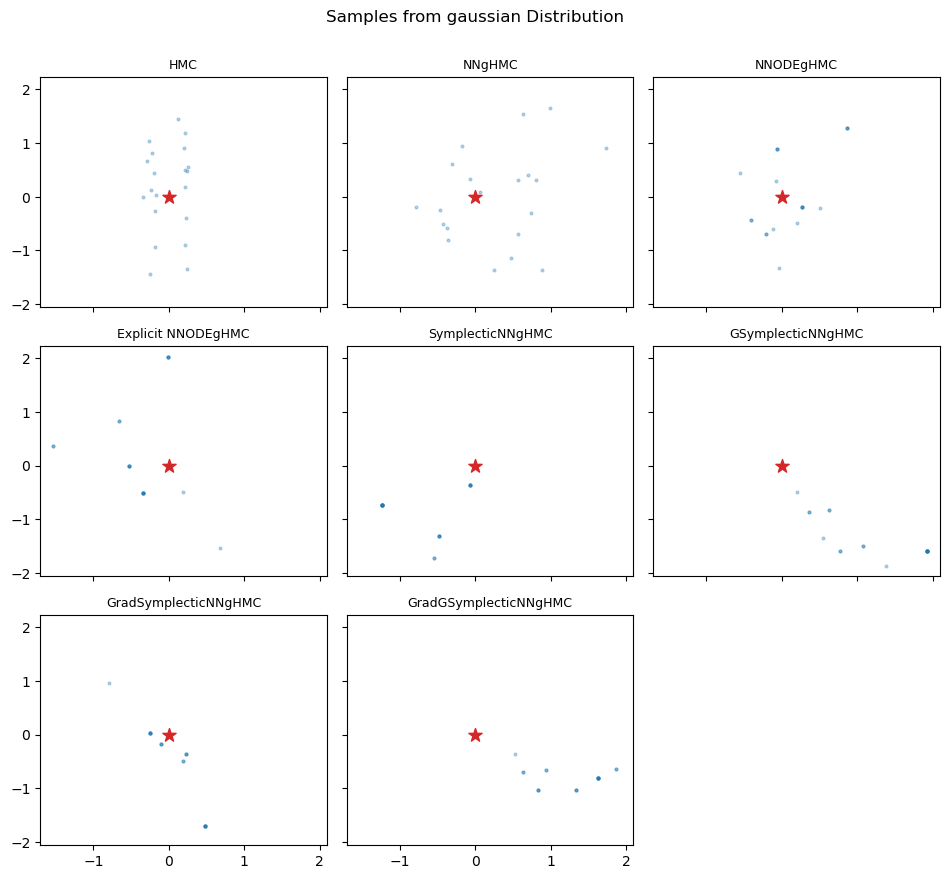
\includegraphics[width=\textwidth]{../experiments/gaussian_samples.png}
\caption{Samples from each method for the multivariate Gaussian. The
integrator-based surrogates reproduce the target. The unsymmetrized symplectic
networks (G-SympNet and both gradient-supervised variants) visibly do not: they
place mass in two lobes with a hole at the mode, which is not a feature of the
target but the bias of an invalid proposal. This is the failure of
\eqref{eq:inv} made visible --- these maps are \emph{exactly} symplectic, so
the defect is not approximate symplecticity but the missing involution
(\Cref{sec:symmetrization}); the symmetrized construction \eqref{eq:psi}
repairs it.}\label{figure:gaussian}
\end{figure*}

\begin{figure*}[!t]
\centering
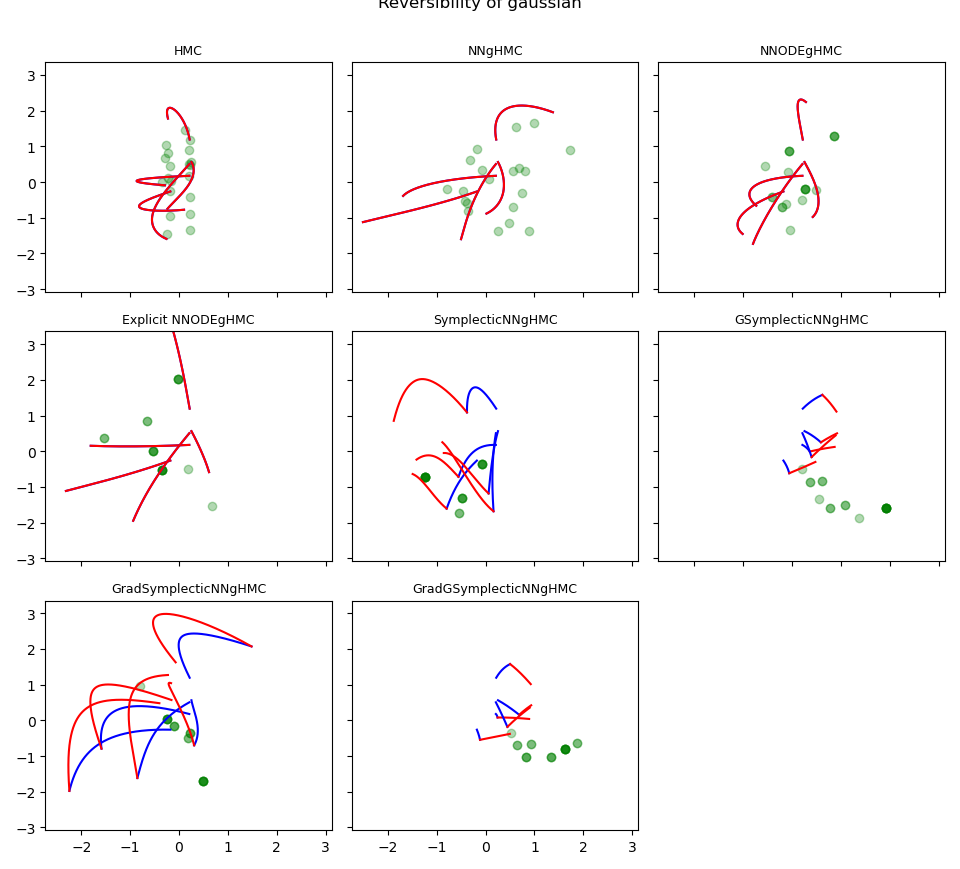
\includegraphics[width=\textwidth]{../experiments/gaussian_reversibility.png}
\caption{Reversibility of the Hamiltonian paths for the multivariate Gaussian: forward trajectories (blue) and the paths obtained by flipping the momentum and integrating back (red), over the sampled positions (green). Quantitative values for every target are given in \Cref{figure:reversibility-stats}. Note that the unsymmetrized symplectic networks sample a split support, so their backward paths start from a region the target does not concentrate on.}\label{figure:gaussian-rev}
\end{figure*}

\begin{figure*}[!t]
\centering
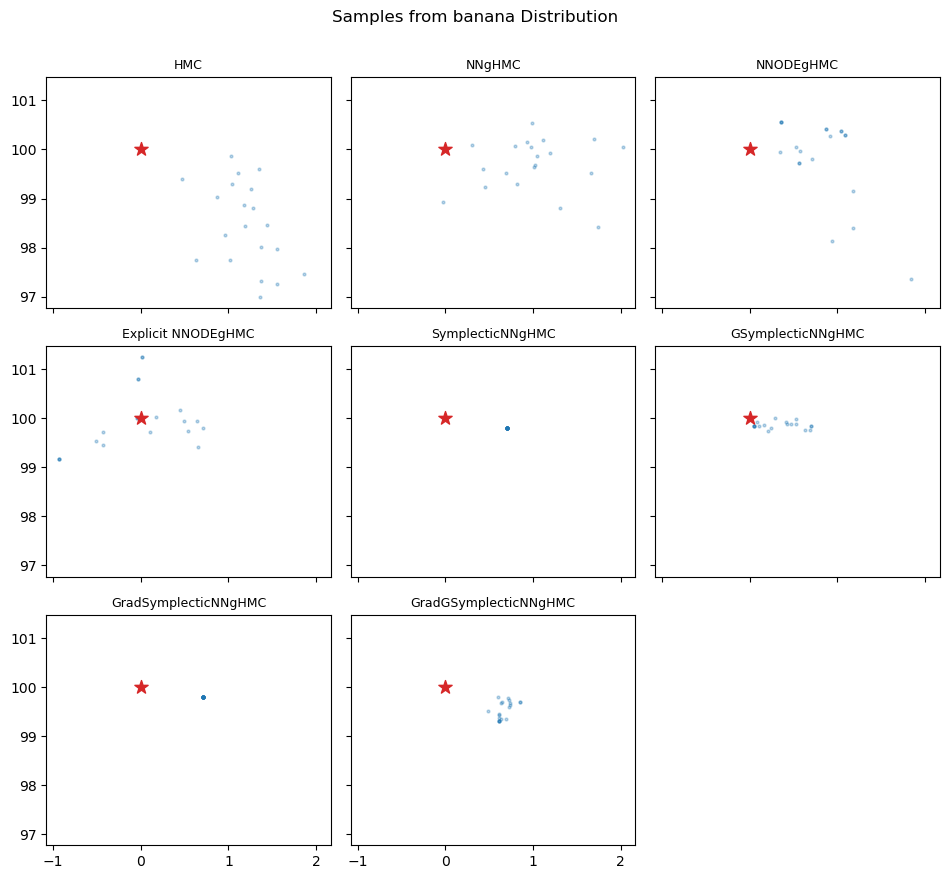
\includegraphics[width=\textwidth]{../experiments/banana_samples.png}
\caption{Samples from each method for the Banana distribution. This target
should not be read as a comparison between methods: exact HMC itself attains an
effective sample size of order $1$ here at $L=5$, $\epsilon=0.1$, so no method
is sampling it adequately. The banana's curvature grows with $\theta_1$, which
caps the stable step size while the marginal scale demands long trajectories ---
a conditioning problem that a fixed identity mass matrix cannot resolve, and one
better addressed by the Riemannian methods of \Cref{sec:symmetrization}.}\label{figure:banana}
\end{figure*}


\begin{figure*}[!t]
\centering
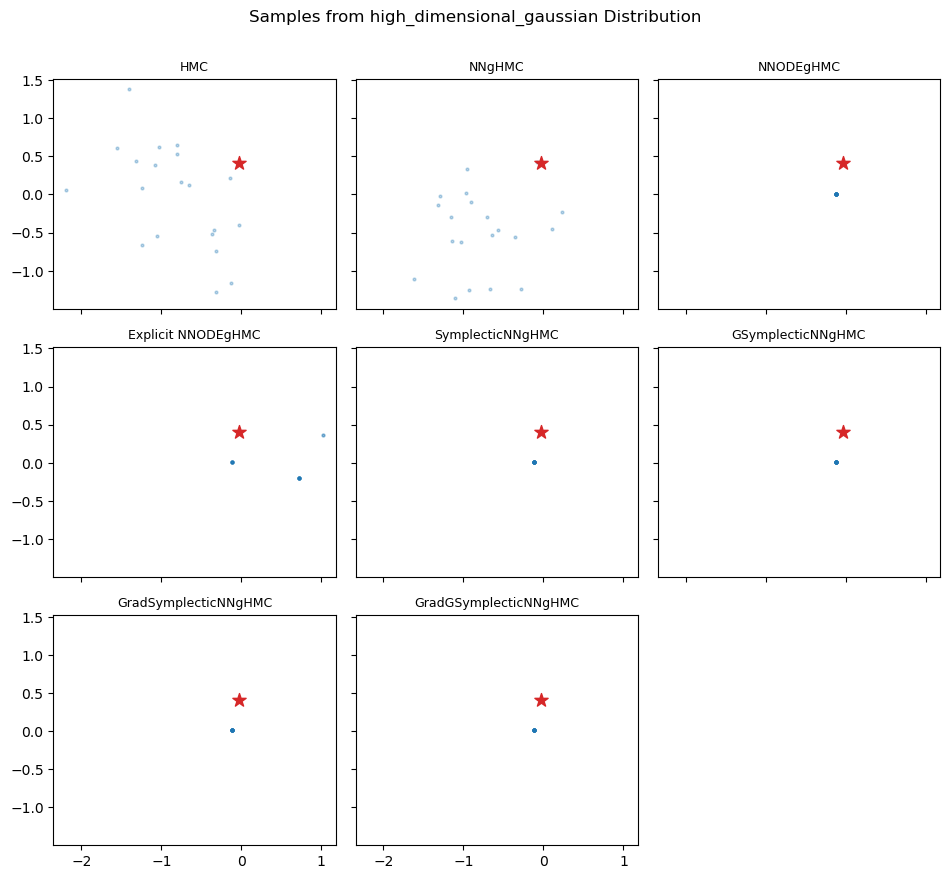
\includegraphics[width=\textwidth]{../experiments/high_dimensional_gaussian_samples.png}
\caption{Samples from each method for the $30$-dimensional Gaussian (first two
coordinates shown).}\label{figure:hdgaussian}
\end{figure*}




\begin{figure*}[!t]
\centering
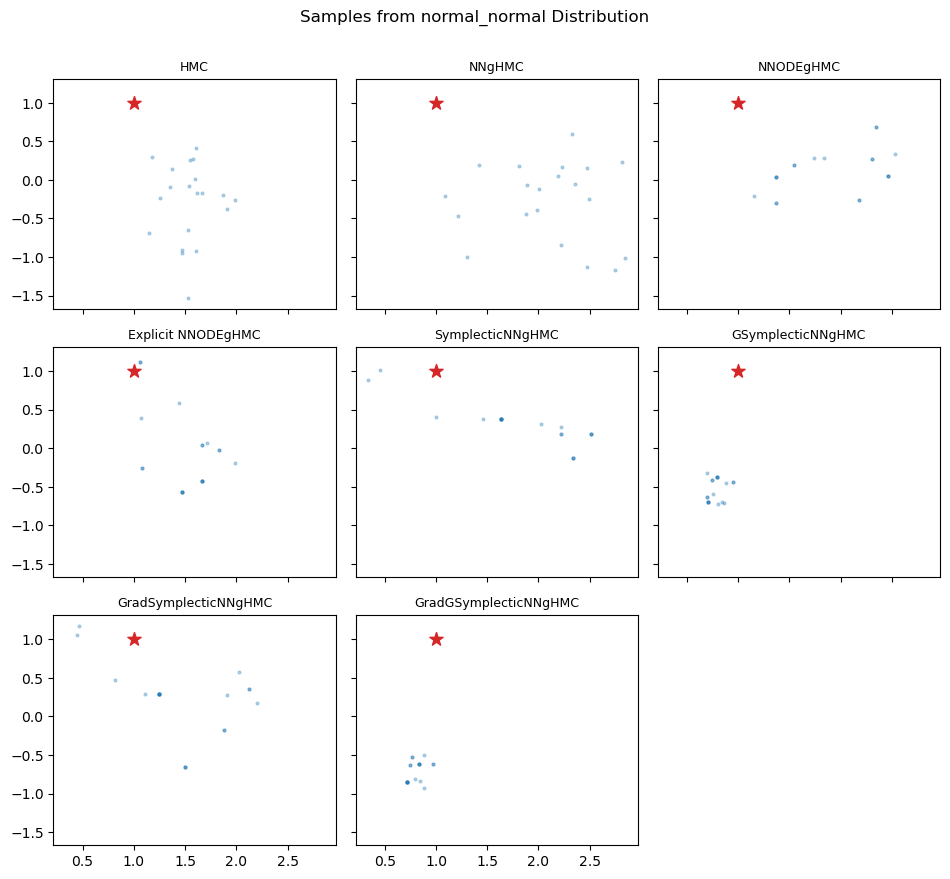
\includegraphics[width=\textwidth]{../experiments/normal_normal_samples.png}
\caption{Samples from each method for the Normal-Gamma posterior.}\label{figure:normal-gamma}
\end{figure*}

\begin{figure*}[!t]
\centering
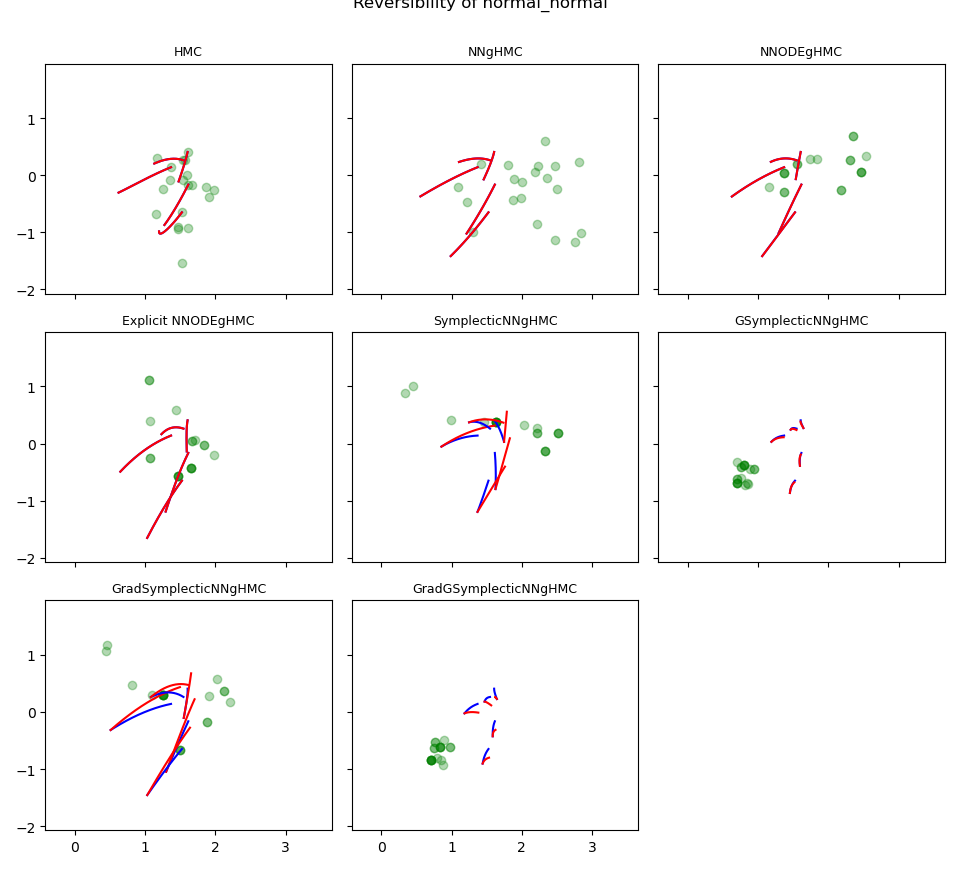
\includegraphics[width=\textwidth]{../experiments/normal_normal_reversibility.png}
\caption{Reversibility of the Hamiltonian paths for the Normal-Gamma distribution: forward trajectories (blue) and the paths obtained by flipping the momentum and integrating back (red), over the sampled positions (green). Quantitative values are given in \Cref{figure:reversibility-stats}.}\label{figure:normal-gamma-rev}
\end{figure*}

\begin{figure*}[!t]
\centering
{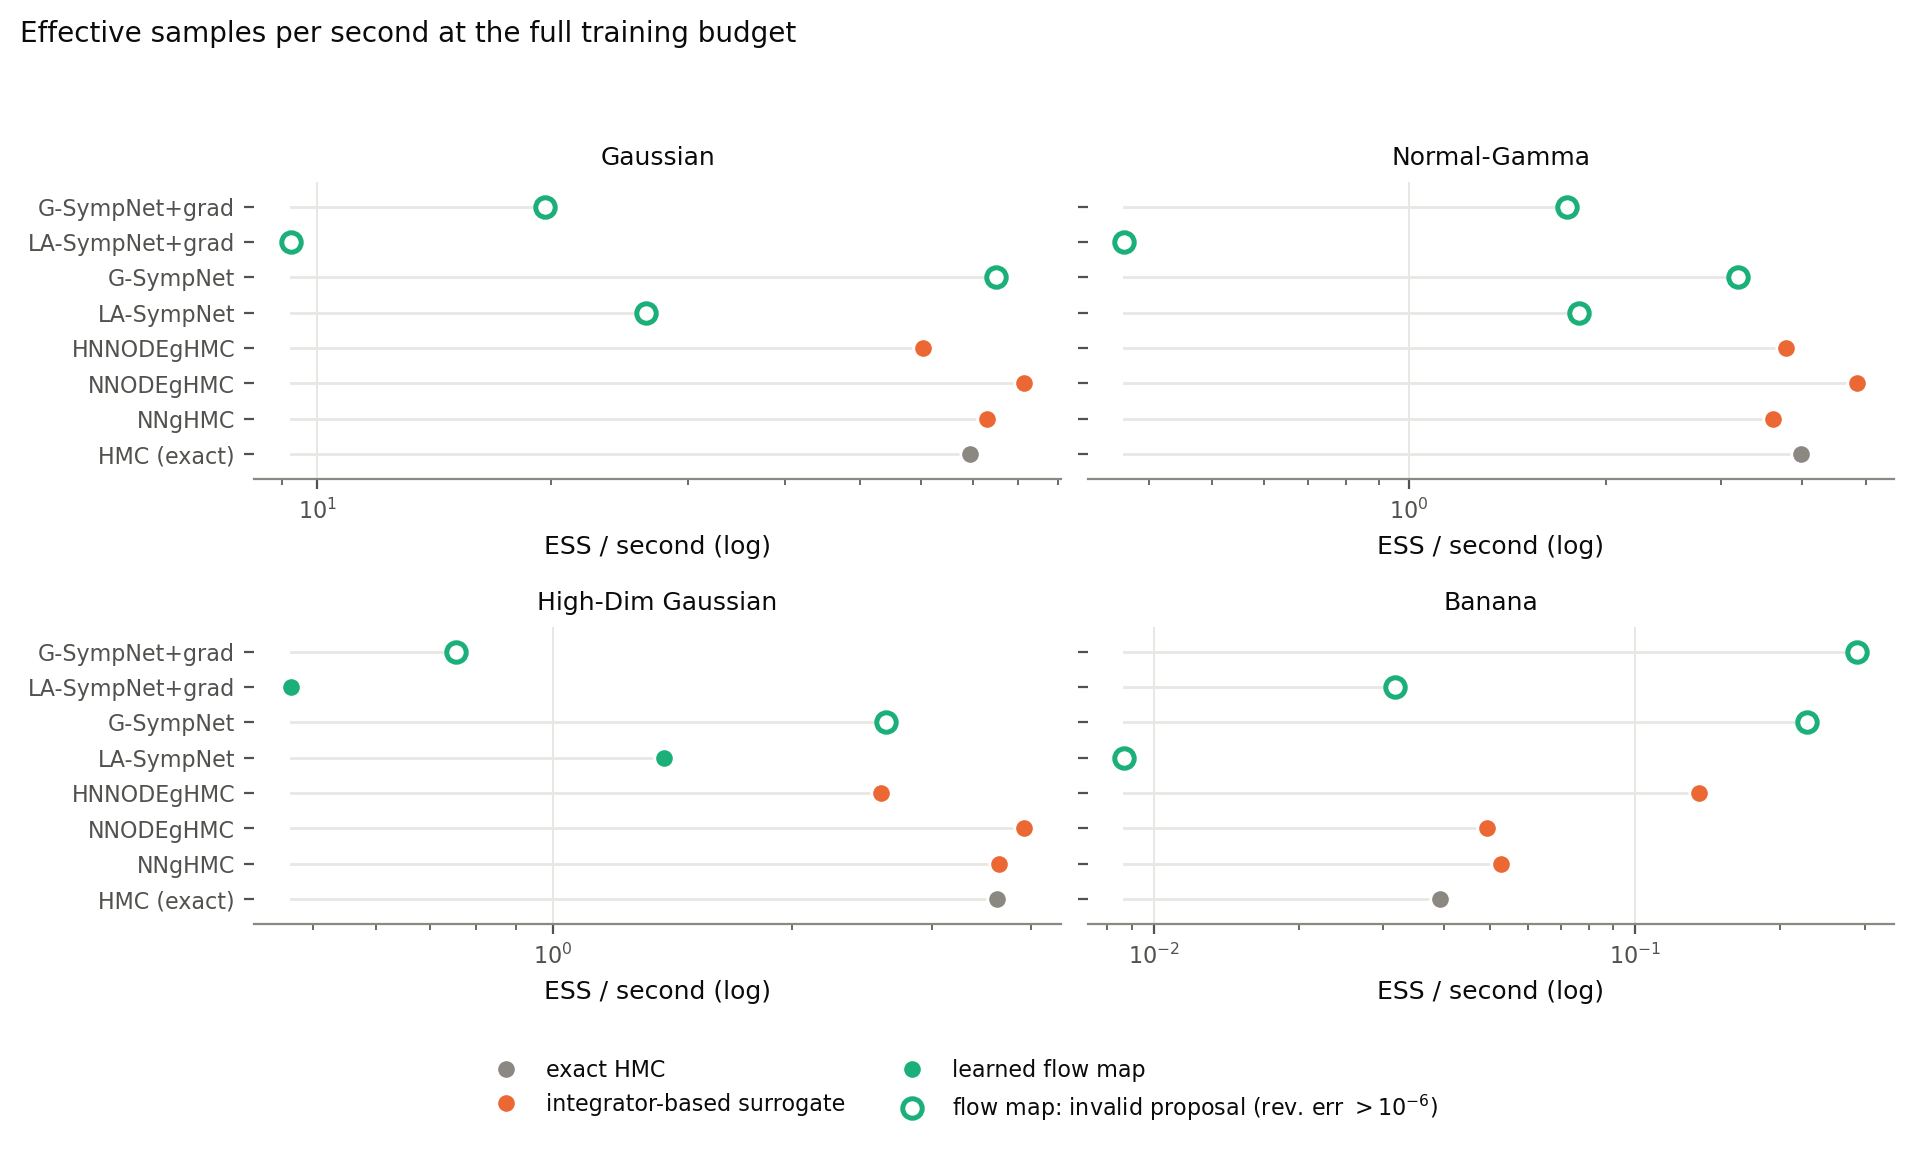
\includegraphics[width=\textwidth]{../experiments/ess_stats.png}}

\caption{Effective samples per second at the full training budget (log scale;
dot plots rather than bars, since a bar encodes magnitude by length from zero
and a log axis has no zero). Markers are coloured by family; unsymmetrized flow
maps whose reversibility error exceeds $10^{-6}$ are drawn as open circles,
because their ESS does not certify a valid sampler. Among methods that are valid
proposals, trajectory-guided NNODEgHMC attains the highest ESS/s on three of the
four targets, modestly ahead of exact HMC ($81.3$ versus $69.3$ on the Gaussian).
The banana column should not be read as a comparison: exact HMC itself achieves
an ESS of order $1$ there, so no method is sampling that target adequately.}\label{figure:ess-stats}
\end{figure*}

\begin{figure*}[!t]
\centering
{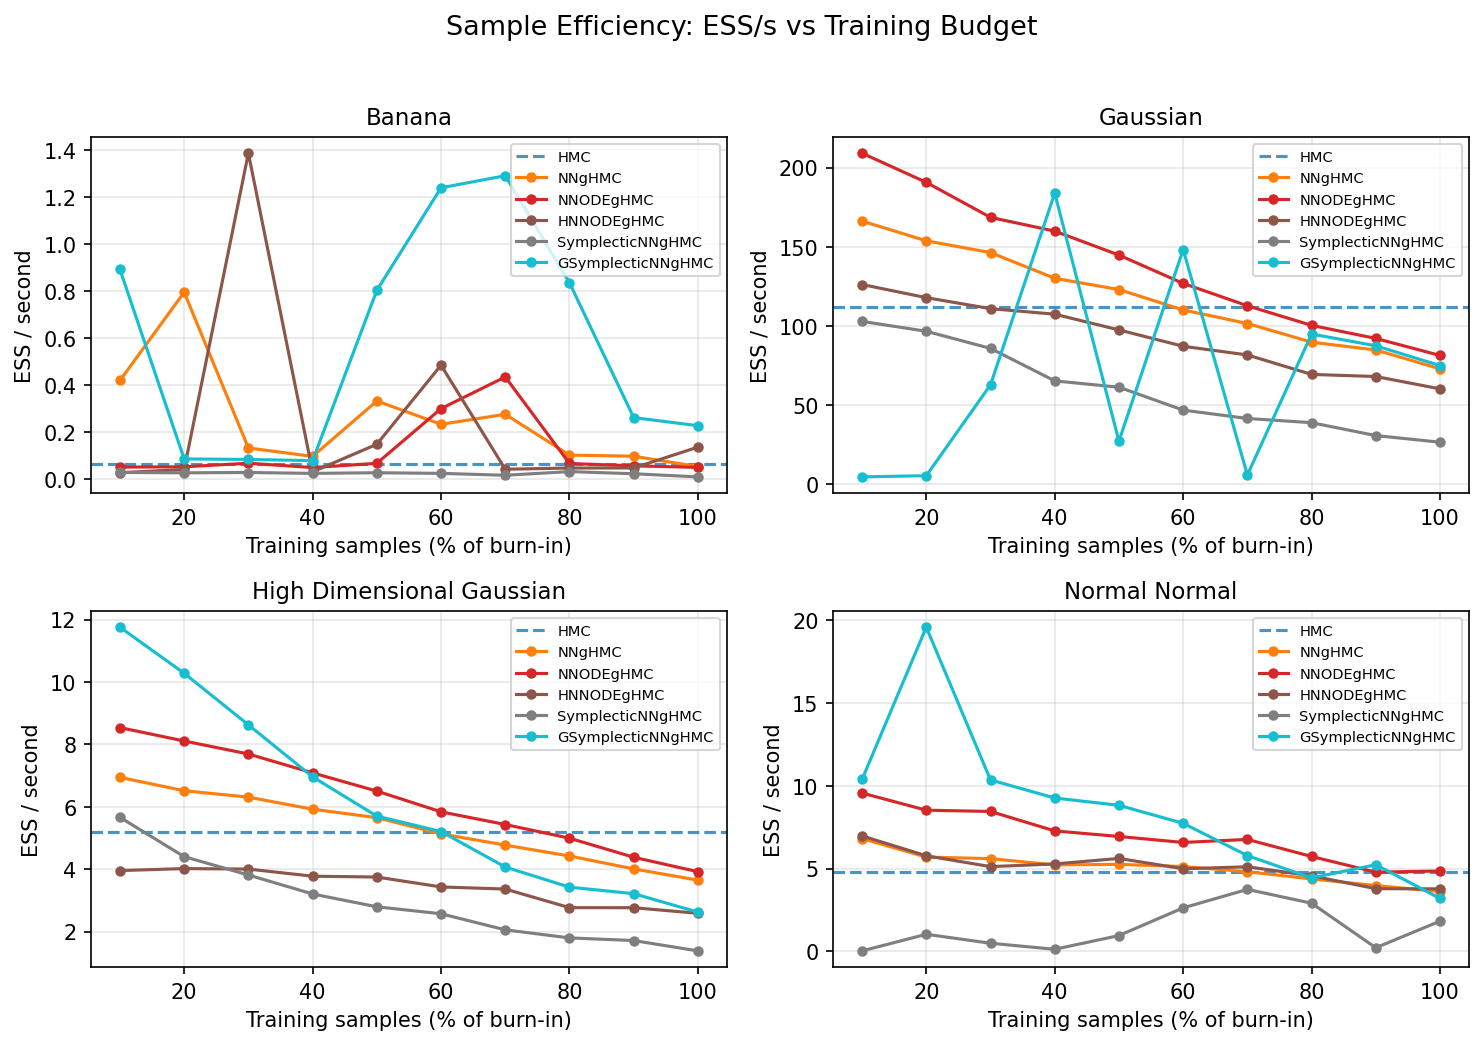
\includegraphics[width=\textwidth]{../experiments/ess_vs_training_size.png}}

\caption{ESS/s as a function of the fraction of burn-in trajectories used for
surrogate training, across all four distributions. NNODEgHMC (trajectory-guided)
reaches competitive ESS/s with substantially fewer training samples than NNgHMC,
supporting the claim that trajectory-level supervision enables more
sample-efficient training. HMC is shown as a dashed reference. SNN methods are
omitted from this panel: as \Cref{figure:reversibility-stats} shows, the
unsymmetrized variants are not valid proposals, so their ESS/s is not
interpretable as sampling efficiency.}\label{figure:ess-vs-training}
\end{figure*}

\begin{figure*}[!t]
\centering
{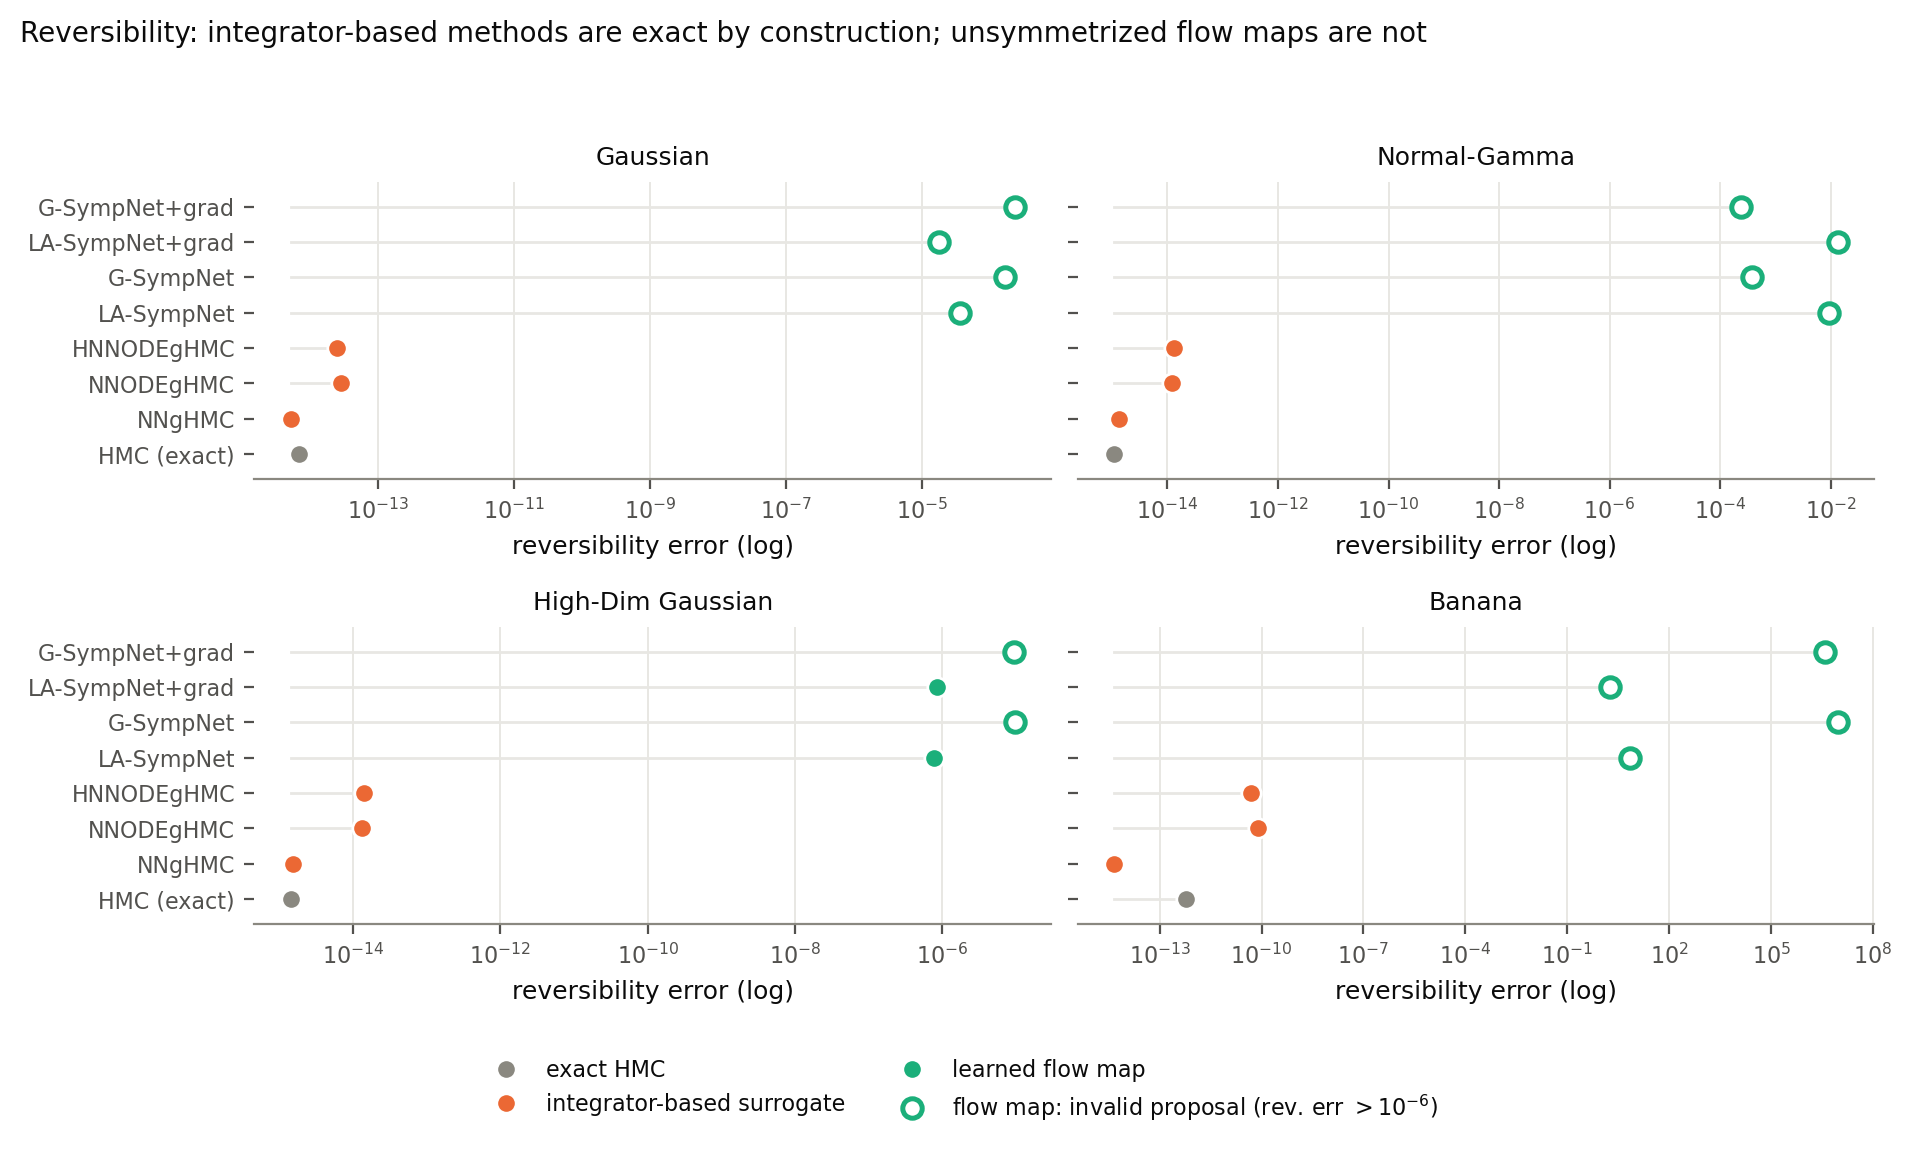
\includegraphics[width=\textwidth]{../experiments/reversibility_stats.png}}



\caption{Reversibility error for each method, log scale. A Hamiltonian flow is
time-reversal symmetric, so flipping the momentum and travelling for $L$ steps
must return the initial position; the error is the distance between the starting
point and the point so reached. The integrator-based methods are exact to
machine precision ($1.3\times10^{-15}$ to $7.7\times10^{-11}$), which is a
property of the integrator and holds for any learned field. The unsymmetrized
SNNs are not: their error spans $7.7\times10^{-7}$ to $9.3\times10^{6}$, i.e.\
up to thirteen orders of magnitude worse. This is a structural deficiency rather
than an approximation error, and it does not diminish with more training data;
see \Cref{sec:symmetrization}.}\label{figure:reversibility-stats}
\end{figure*}



\begin{figure*}[!t]
\centering
{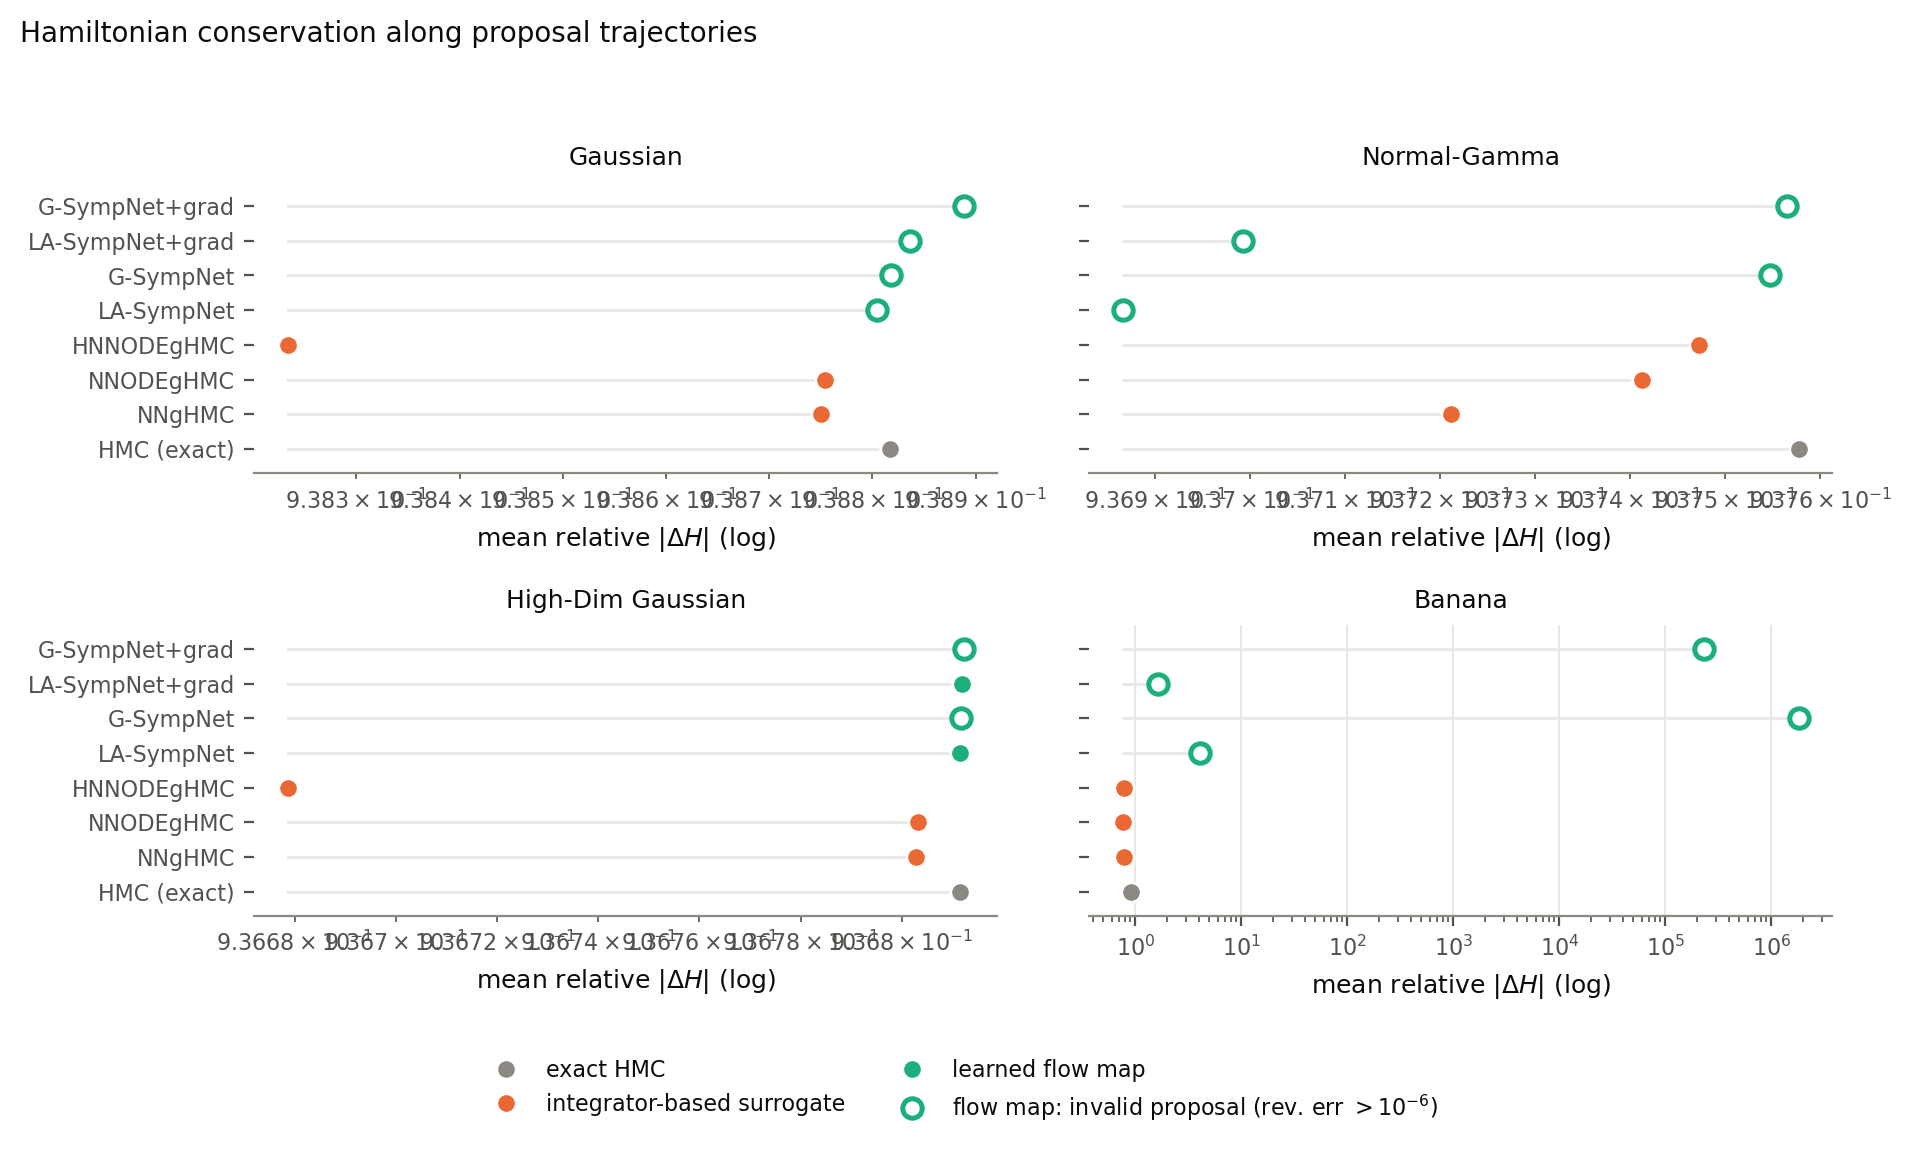
\includegraphics[width=\textwidth]{../experiments/hamiltonian_conservation.png}}



\caption{Mean relative change in the Hamiltonian along proposal trajectories,
log scale. A symplectic integrator applied to a learned field conserves a
modified Hamiltonian and so shows little systematic drift; the integrator-based
surrogates behave accordingly. The unsymmetrized SNNs show substantially larger
drift. We caution that conservation and reversibility are distinct properties:
a map can be exactly symplectic, and hence volume preserving, while failing the
involution condition that the Metropolis correction requires
(\Cref{figure:reversibility-stats}).}\label{figure:hamiltonian-stats}
\end{figure*}

\section{Discussion and Future Work}
Experiments in the Hamiltonian Monte Carlo setting for a few distributions showed that adding a trajectory deviation penalty to traditional NNgHMC \cite{Li_2019} allows for more efficient training; as shown in \Cref{figure:ess-vs-training}, fewer training samples were needed to produce proposals of similar quality. However, as the NNODEgHMC models are trained using Neural ODE methods, longer trajectory length could prove to be computationally costly. The benefit of gradient based models which are integrated with leapfrog integrators was clearly shown; they behave with proper Hamiltonian dynamics, if given enough training samples.

On the contrary, directly learning the flow of the Hamiltonian through SNNs
proved to be an interesting experiment; SNNs were able to produce quality
samples from the posterior while approximating Hamiltonian dynamics. Unlike
the integrator-based surrogates, whose training cost is independent of
trajectory length, the SNN objective grows quadratically in $L$ through the
pair construction, which mini-batching mitigates but does not remove.

Two limitations of the flow-learning approach are worth separating. The first
is statistical: what the SNN must learn is a map on the full $2D$-dimensional
phase space, parameterized by time, whereas the gradient-based surrogates learn
a field on the $D$-dimensional position space alone, from labels the warm-up
phase already produces. The second is structural, and is the more consequential
of the two: as shown in \Cref{sec:symmetrization}, an unmodified SNN supplies
volume preservation but not involutivity, so it is not a valid Metropolis
proposal at all, and its bias does not diminish with additional training data.
The symmetrized construction $\Psi_t$ repairs this exactly and at no cost in
parameters, and it is the form in which we would recommend the architecture be
used. We caution that $\Psi_t$ evaluates the underlying network twice, so
comparisons against unsymmetrized baselines must control for effective depth
rather than block count.

Approximating RMHMC is a natural extension of this work, and one where the
economics are more favorable: because Riemannian trajectories require a metric
tensor --- and hence second derivatives of the log density --- at every stage of
the integrator, the cost per exact trajectory is far higher, so a surrogate has
correspondingly more to save. Two aspects transfer directly. Trajectories are
generated with the explicit integrator of \cite{Tao_2016} on the augmented
state, and the complete phase-space field $(\partial_p H, -\partial_q H)$ is
recorded during warm-up at no meaningful additional cost, since the integrator
already forms it; that field supplies gradient supervision for the
non-separable case exactly as $\nabla \log p$ does in the separable one.
Because SNNs approximate arbitrary symplectic maps, the flow-learning
architecture requires no modification whatsoever for the non-separable
setting --- only the source of the training trajectories changes.





\clearpage
\clearpage
\bibliography{bibliography}
\bibliographystyle{icml2024}



%%%%%%%%%%%%%%%%%%%%%%%%%%%%%%%%%%%%%%%%%%%%%%%%%%%%%%%%%%%%%%%%%%%%%%%%%%%%%%%
%%%%%%%%%%%%%%%%%%%%%%%%%%%%%%%%%%%%%%%%%%%%%%%%%%%%%%%%%%%%%%%%%%%%%%%%%%%%%%%
% APPENDIX
%%%%%%%%%%%%%%%%%%%%%%%%%%%%%%%%%%%%%%%%%%%%%%%%%%%%%%%%%%%%%%%%%%%%%%%%%%%%%%%
%%%%%%%%%%%%%%%%%%%%%%%%%%%%%%%%%%%%%%%%%%%%%%%%%%%%%%%%%%%%%%%%%%%%%%%%%%%%%%%
\newpage
\appendix

%%%%%%%%%%%%%%%%%%%%%%%%%%%%%%%%%%%%%%%%%%%%%%%%%%%%%%%%%%%%%%%%%%%%%%%%%%%%%%%
%%%%%%%%%%%%%%%%%%%%%%%%%%%%%%%%%%%%%%%%%%%%%%%%%%%%%%%%%%%%%%%%%%%%%%%%%%%%%%%






\end{document}





% This document was modified from the file originally made available by
% Pat Langley and Andrea Danyluk for ICML-2K. This version was created
% by Iain Murray in 2018, and modified by Alexandre Bouchard in
% 2019 and 2021 and by Csaba Szepesvari, Gang Niu and Sivan Sabato in 2022.
% Modified again in 2023 and 2024 by Sivan Sabato and Jonathan Scarlett.
% Previous contributors include Dan Roy, Lise Getoor and Tobias
% Scheffer, which was slightly modified from the 2010 version by
% Thorsten Joachims & Johannes Fuernkranz, slightly modified from the
% 2009 version by Kiri Wagstaff and Sam Roweis's 2008 version, which is
% slightly modified from Prasad Tadepalli's 2007 version which is a
% lightly changed version of the previous year's version by Andrew
% Moore, which was in turn edited from those of Kristian Kersting and
% Codrina Lauth. Alex Smola contributed to the algorithmic style files.

